% PAKETE UND DOKUMENTKONFIGURATION
\documentclass[11pt, a4paper]{article}

% Encoding für Umlaute
\usepackage[utf8]{inputenc}
\usepackage[T1]{fontenc}

% Silbentrennung
\usepackage[ngerman]{babel}

% erweiterte Matheumgebungen und Formelnummer mit Sectionnummer
\usepackage{amsmath}
\numberwithin{equation}{section}

% Braket Notation
\usepackage{braket}
\usepackage{isotope}
\usepackage[version=3]{mhchem}

% zusätzliche mathematische Schriftarten
\usepackage{amsfonts}

% verschiedene mathematische Symbole
\usepackage{amssymb}

% Einheiten setzen z.B. \SI{10}{\kilo\gram\meter\per\second\squared}
% Fehler: \SI{10 +- 0,2e-4}{\metre}
\usepackage{siunitx}
\sisetup{
  output-decimal-marker={,},
  separate-uncertainty
}

% Einheitendefinitionen
\DeclareSIUnit{\skt}{Skt.}
\DeclareSIUnit{\gauss}{G}
\DeclareSIUnit{\division}{div.}

% Operatordefinitionen
\DeclareMathOperator{\erf}{erf}

% Randbreiten
\usepackage[left=3.5cm,right=3.5cm,top=3cm,bottom=3cm,twoside]{geometry}

% Bilder einfügen
\usepackage{graphicx}

% Verweise innerhalb des Dokuments
\usepackage{hyperref}
\hypersetup{
	colorlinks = true,
	allcolors = {black}
}

% bessere Tabellenlayouts
\usepackage{booktabs}
\usepackage{multirow}
\usepackage{multicol}

% Seitenlayout (Kopfzeile)
\usepackage{fancyhdr}

% Float Barriers
\usepackage{placeins}

% Pakete für gedrehte Subfigures
\usepackage{caption}
\usepackage{subcaption}
\usepackage{rotating}

% Paket für textumflossene Abbildungen und Tabellen
\usepackage{wrapfig}

\usepackage{float}

% Caption-Setup
\captionsetup{font={small}}
\renewcommand{\thefigure}{\thesection.\arabic{figure}}
\renewcommand{\thesubfigure}{\alph{subfigure}}
\renewcommand{\thetable}{\thesection.\arabic{table}}
\renewcommand{\thesubtable}{\alph{subtable}}

% Manuelle Silbentrennung
\hyphenation{Sig-nal-ver-hal-ten Szin-til-la-tions-de-tek-tors}

% Tiefe des Inhaltsverzeichnisses (Level: 1 sections, 2 subsections,
% 3 subsubsections)
\setcounter{tocdepth}{3}

% FANCYHDR SETUP
\pagestyle{fancy}
\fancyhead[EL,OR]{\thepage}
\fancyhead[ER]{\leftmark}
\fancyhead[OL]{\rightmark}
\setlength{\headheight}{13.6pt}

\renewcommand{\sectionmark}[1]{
\markboth{\thesection{} #1}{\thesection{} #1}
}
\renewcommand{\subsectionmark}[1]{
\markright{\thesubsection{} #1}
}

\newcommand{\ptt}{Peak-to-Total-Verhältnis}
\newcommand{\co}{\isotope[60]{Co}}
\newcommand{\cs}{\isotope[137]{Cs}}
\newcommand{\eu}{\isotope[152]{Eu}}

% DOKUMENTINFORMATIONEN
\title{P529 \\ Dosimetrie und Abschirmung}

\author{Christopher Deutsch\footnote{christopher.deutsch@uni-bonn.de} \and Christian Bespin\footnote{christian.bespin@uni-bonn.de}}

\date{\today}

\begin{document}

\begin{titlepage}

\maketitle

% DURCHFÜHRUNGSDATUM UND TUTOR
\begin{center}
\begin{tabular}{l r}
Durchführung: & 4./5. Mai 2015 \\
Gruppe: & $\alpha$ 6 \\
Tutor: & Marcus Gruener
\end{tabular}
\end{center}

% ZUSAMMENFASSUNG
\begin{abstract}
\noindent
\end{abstract}

\end{titlepage}

% INHALTSVERZEICHNIS
\tableofcontents
% Neue Seite nach TOC
\newpage

% INHALT VERSUCHSPROTOKOLL

\section{Einführung}

\section{Theorie}
\subsection{Röntgenstrahlung}
Als Röntgenstrahlung wird der Teil des elektromagnetischen Spektrums mit Photon-Energien zwischen \SI{100}{\electronvolt} und \SI{100}{\kilo\electronvolt} bezeichnet, wobei diese Grenzen nicht scharf sind und deshalb oft hinsichtlich der Strahlungsquelle eine Einordnung vollzogen wird.

\subsubsection{Erzeugung}
\label{sec:röntgenerzeugung}
Es gibt zwei typische Erzeugungsmethoden von Röntgenstrahlung, welche auf dem Beschuss eines \emph{Targets} mit einem hochenergetischen Elektronenstrahl bestehen.
Die beiden Strahlungsarten, welche in der Praxis oft zusammen auftreten, sind:
\begin{itemize}
	\item \textbf{Bremsstrahlung:} Die bei der Streuung der geladenen Elektronen an den Kernen des Targets vollzogene Geschwindigkeitsänderung des Elektrons, führt zur Emission eines Photons.
	Das so entstandene Spektrum ist kontinuierlich, wobei die maximale Photonenenergie gegeben ist durch die kinetische Energie der einfallenden Elektronen, welche durch deren Beschleunigungsspannung $U$ gegeben ist.
	Überträgt das Elektron seine gesamte Energie auf ein einzelnes Photon:
	\begin{align}
	&E_\mathrm{kin. e^-} = h \cdot \nu_\mathrm{max} = \frac{hc}{\lambda_\mathrm{min}}
	\end{align}
	so ist diese Grenze gegeben durch das \textbf{Duane-Hunt-Gesetz}
	\begin{align}
	\lambda_\mathrm{min} = \frac{h c}{e U}
	\label{eq:duane_hunt}
	\end{align}
	Eine Quelle für reine Bremsstrahlung sind Synchrotronstrahlungsquellen.
	
	\item \textbf{charakteristische Strahlung:} Die einfallende hochenergetische Elektronenstrahlung ionisiert ein Elektron der inneren Schale eines Targetatoms.
	Dadurch entsteht ein freier Zustand, welcher durch ein Elektron einer weiter äußeren Schale eingenommen werden kann.
	Durch den Übergang wird ein Photon emittiert, dessen Energie gleich der Energiedifferenz der beiden Zustände ist.
	Aufgrund dieser Abhängigkeit von der elektronisches Struktur des Targetatoms, ist das emittierte, diskrete Spektrum charakteristisch für das verwendete (Target)-Material.
	Außerdem weist das emittierte Spektrum die Aufspaltung der Energieniveaus aufgrund von Fein- und Hyperfeinstruktur auf.
\end{itemize}
In der Praxis treten beide Effekte bei der Erzeugung von Röntgenstrahlen in sogenannten Röntgenröhren auf, wie in Abbildung \ref{fig:spektrum} zu sehen ist.
\begin{figure}[ht]
	\centering
	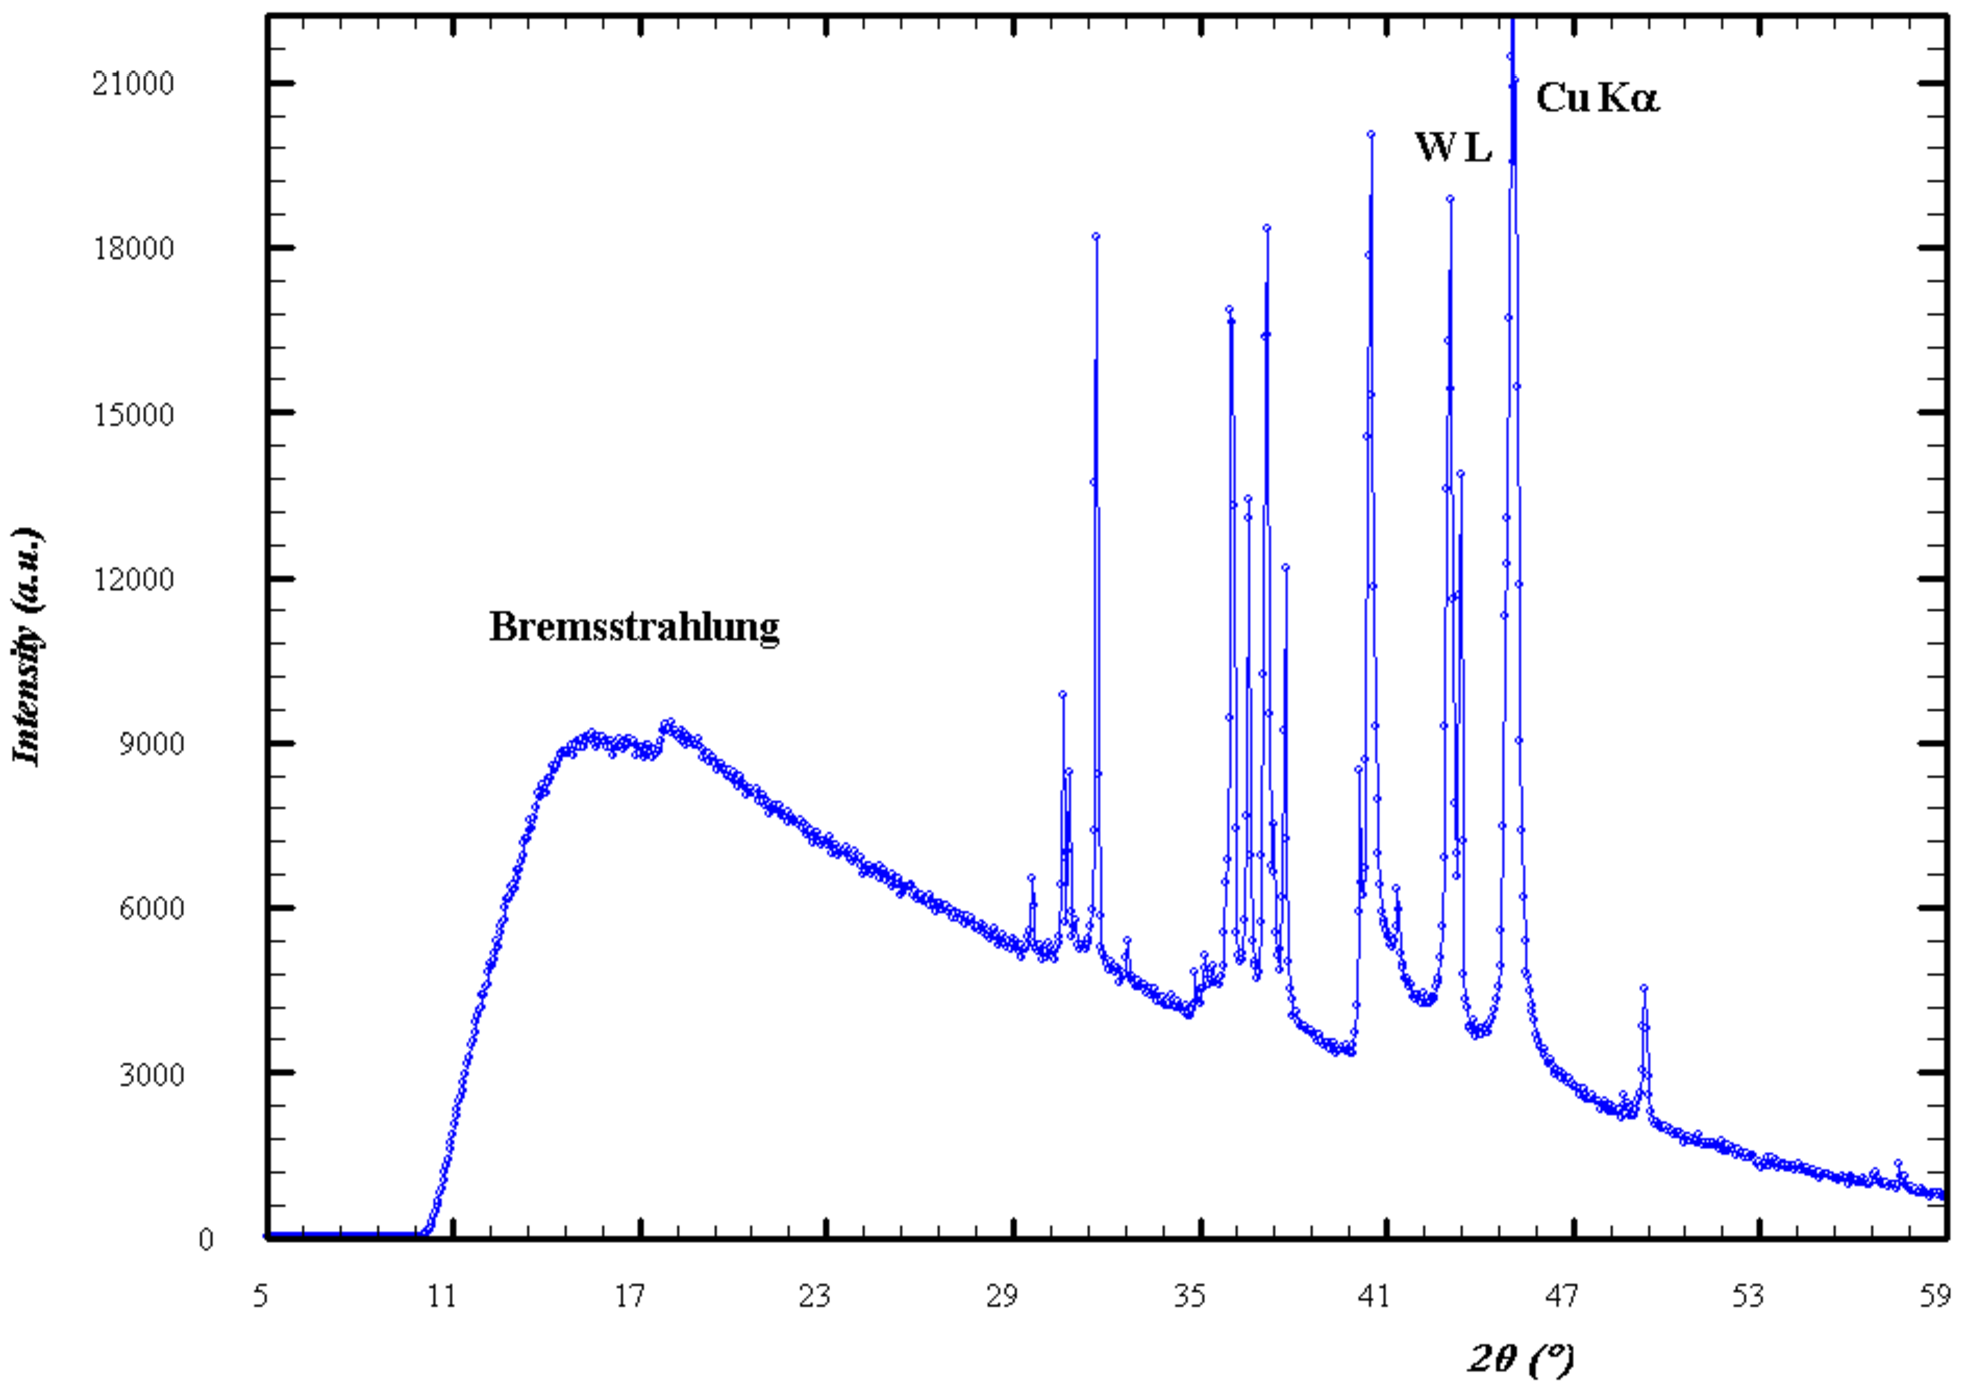
\includegraphics[width=1\textwidth]{./figures/Tube_Cu_LiF.pdf}
	\caption{Charakteristisches Spektrum einer Kupferanode nach Bragg-Reflexion an einem LiF-Kristall. Der Untergrund entsteht aufgrund der emittierten Bremsstrahlung der in der Anode gestreuten Elektronen. Auf diesem liegt das charakteristische Röntgenspektrum der Anode. Quelle: \url{http://commons.wikimedia.org/wiki/File:Tube_Cu_LiF.PNG} (Letzter Zugriff: 13. November 2014)}
	\label{fig:spektrum}
\end{figure}

Eine \textbf{Röntgenröhre} (schematisch in Abbildung \ref{fig:roehre}) besteht aus einem evakuierten Glaskolben mit einer Anordnung von geheizter Kathode und Anode aus Targetmaterial.
Zwischen Kathode und Anode wird die Beschleunigungsspannung $U$ angelegt, sodass beim Heizen der Kathode mit der Heizspannung $U_\mathrm{Heiz}$ aufgrund des glühelektrischen Effekts ein Teil der Elektronen die Austrittsarbeit der Kathode überwinden kann und durch die Beschleunigungsspannung $U$ in Richtung der Anode beschleunigt werden.
Nachdem die Beschleunigungsspannung $U$ durchlaufen wurde, treffen die Elektronen mit der Energie $e U$ auf das Anodenmaterial und erzeugen dabei Bremsstrahlung sowie charakteristische Strahlung, welche durch ein für Röntgenstrahlung durchlässiges Fenster im Glaskolben aus der Röhre austreten können.
\begin{figure}[ht]
	\centering
	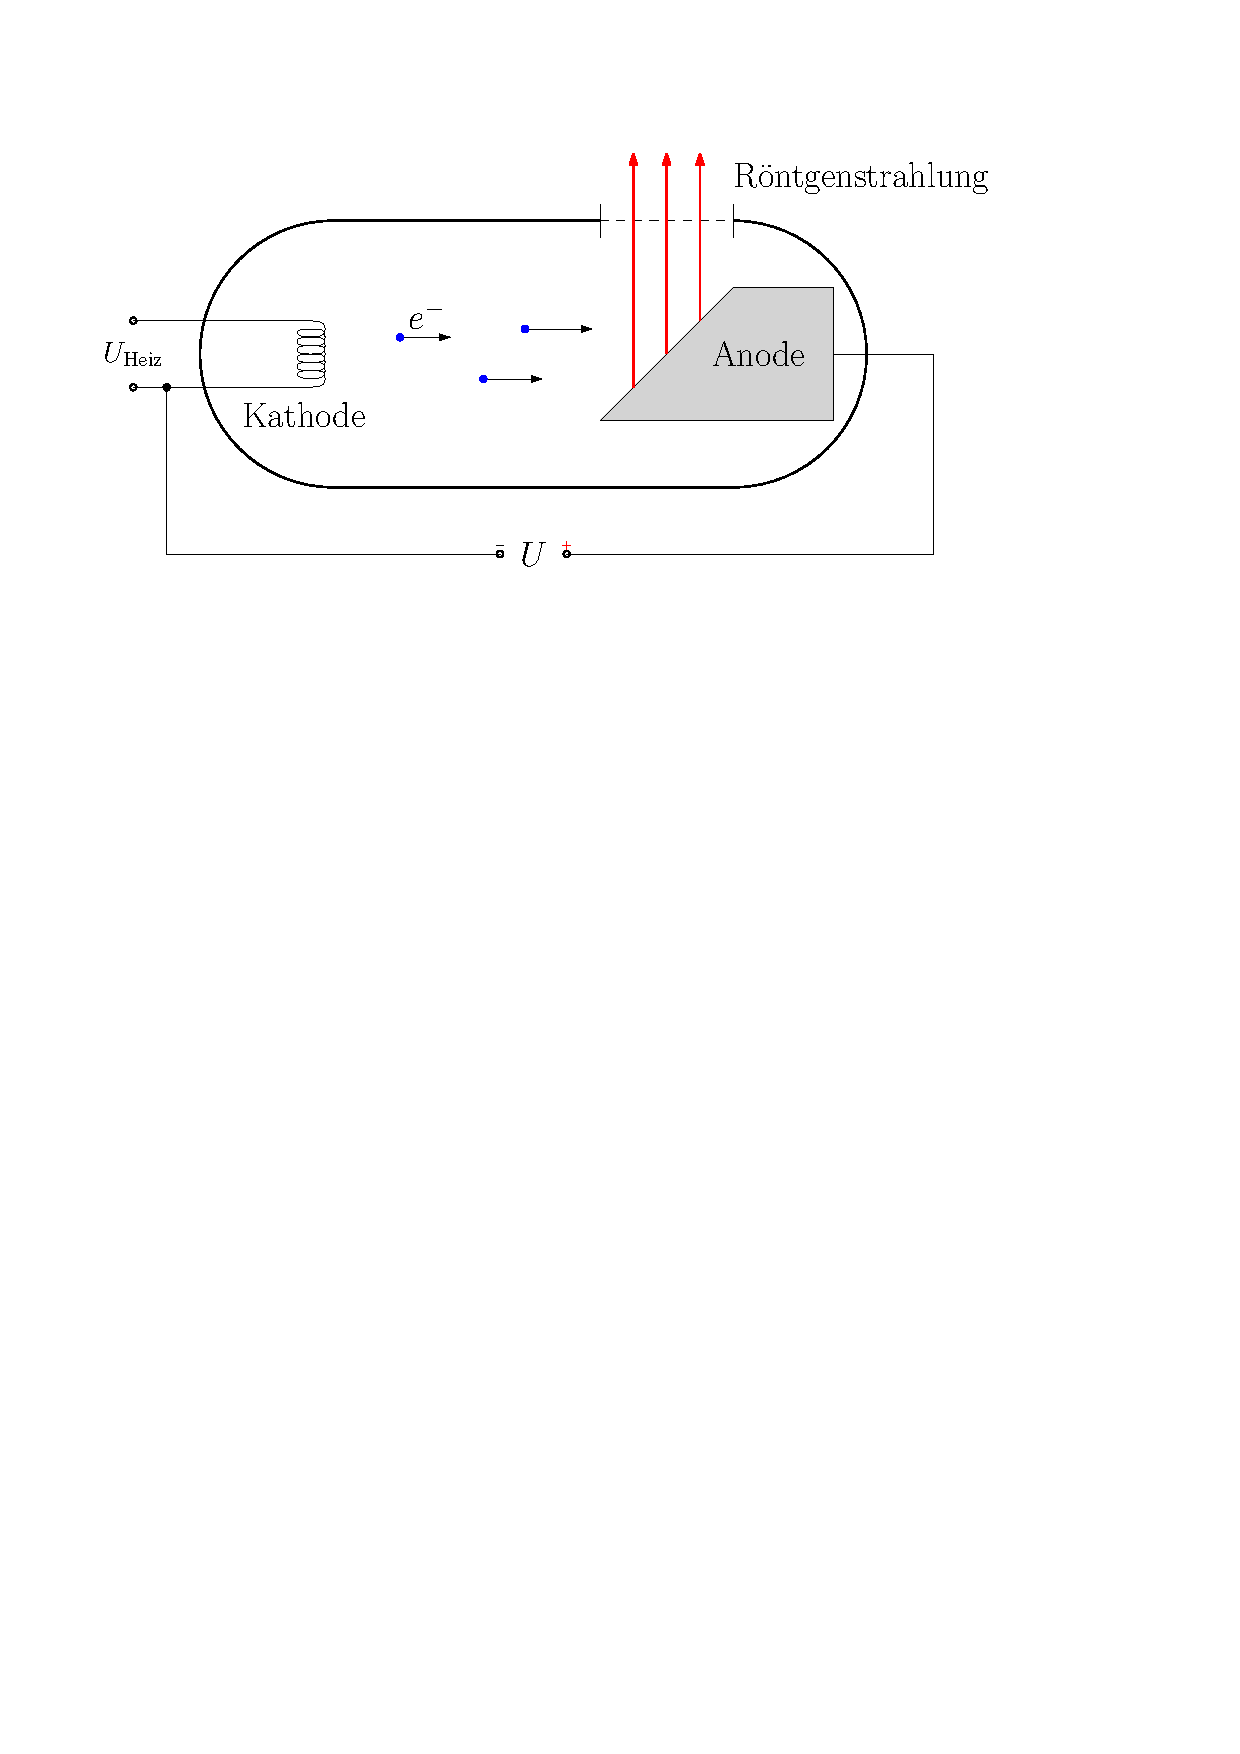
\includegraphics[width=0.75\textwidth]{./figures/roentgenroehre.pdf}
	\caption{schematischer Aufbau einer Röntgenröhre}
	\label{fig:roehre}
\end{figure}

\subsection{Röntgenstrahlung}

\subsubsection{Erzeugung und Nachweis}
NACHWEIS:
\begin{itemize}
	\item \textbf{Lumineszenz:} Bestimmte Stoffe werden durch Röntgenstrahlung zur Emission von Licht angeregt.
	
	\item \textbf{Photographischer Effekt:} Röntgenstrahlung schwärzt einen Röntgenfilm direkt.
	
	\item \textbf{Szintillationszähler, Halbleiterdetektoren, Geigerzähler}
\end{itemize}

\subsubsection{kontinuierliches und charakteristisches Röntgenspektrum}


\subsection{Geiger-Müller-Zählrohr}
Das Geiger-Müller-Zählrohr besteht aus einem Metallzylinder, der die Kathode darstellt und einem Draht im Inneren des Zylinders, der die Anode bildet.
Der Zylinder ist mit einem Gas unter hohem Druck gefüllt, wobei meistens ein Edelgas verwendet wird, da dieses keine negativen Ionen bildet, die den Betrieb stören können.
Bei Eintritt von Teilchen in das Zählrohr werden die Gasatome im Inneren ionisiert und so freie Elektronen und positiv geladene Ionen erzeugt.
Durch die zwischen Draht und Zylindermantel anliegende Spannung werden die Elektronen zum Draht beschleunigt, die Ionen aufgrund ihrer höheren Masse deutlich langsamer zum Mantel hin.

Für den Betrieb ist die angelegte Gleichspannung zwischen Anode und Kathode entscheidend:
Bei geringer Spannung können die freien Elektronen auf der Beschleunigungsstrecke wieder mit den Ionen rekombinieren, wodurch der gemessene Stromimpuls nur von den Elektronen erzeugt wird, die die Anode erreichen.
So kann keine verlässliche Aussage über die einfallende Strahlung gemacht werden (\emph{Rekombinationsbereich}).
Erst ab einer bestimmten Gleichspannung ($\sim \SI{100}{\volt}$) erreichen alle Elektronen die Anode, womit dann die von der Strahlung im Zählrohr abgegebene Energie gemessen wird (\emph{Ionisationskammer}).
Erhöht man die Spannung weiter erreicht man den \emph{Proportionalitätsbereich}.
Hier werden die Elektronen so stark beschleunigt, dass sie auf dem Weg zum Draht genug Energie gewinnen, um weitere Gasatome zu ionisieren.
So entsteht ein Lawineneffekt, der den gemessenen Stromimpuls deutlich vergrößert (bei $n$ Elektronen pro Lawine ist dieser $n$-mal größer) und so genauere Messungen als in der Ionisationskammer ermöglicht.
Beim \emph{Geiger-Müller-Bereich} ist die angelegte Spannung so hoch, dass die Elektronen, ähnlich wie im Proportionalitätsbereich, weitere Atome ionisieren können, und dass die dabei entstandenen Elektronen wieder Atome ionisieren.
Der Lawineneffekt wird also deutlich verstärkt und eine selbstständige Gasentladung ausgelöst.
Diese endet erst, wenn sich durch die entstandenen, positiv geladenen Ionen, die (langsam) zum Mantel des Zylinders beschleunigt werden, eine Raumladungszone im Rohr ausbildet, die die Feldstärke verringert.
Zur Auslösung wird nur ein einzelnes Ereignis benötigt, wodurch das Geiger-Müller-Zählrohr maximale Empfindlichkeit besitzt.
Die gemessenen Stromimpulse sind durch die hohe Beschleunigungsspannung, die die Elektronen erfahren, alle gleich groß, es wird also nur die Anzahl und nicht die Energie der einfallenden Strahlung gemessen.
Durch den angesprochenen Effekt der selbstständigen Gasentladung hat das Geiger-Müller-Zählrohr eine s.g. \emph{Totzeit}, welche beschreibt, wie lange keine neu einfallende Strahlung gemessen werden kann, da die Gasatome vorher beinahe alle ionisiert sind und erst wieder mit den Elektronen rekombinieren müssen.

\subsubsection{Aufbau}

\subsubsection{Funktionsweise}

\subsubsection{Totzeit und Totzeitkorrektur}
Endliche Zeit des Detektors ein Signal zu verarbeiten lässt ihn insensitiv für neue Ereignisse.
Man unterscheidet zwischen Paralysierenden und Nicht-Paralysierenden Systemen.
Bei nicht-paralysierendem Verhalten führt ein zweites Ereignis lediglich zum Verlust dieses Ereignisses.
Bei paralysierendem Verhalten führt ein zweites Event zum "Neustart" der Totzeit.
Bei semi-paralysierendem Verhalten erhöht ein zweites Event lediglich die Zeit in der der Detektor nicht sensitiv ist (aber nicht um die Länge der Totzeit).

(Cite Leo)Unter Annahme eines nicht paralysierenden Systems (Totzeit: $\tau$) mit der wahren Count-Rate $m$ und der vom Detektor gezählten Anzahl der Events $k$ in einer Zeit $T$.
Da jeder Count eine Totzeit auslöst ergibt sich die gesamte Totzeit zu:
\begin{align}
	\tau_\mathrm{ges.} = k \cdot \tau
\end{align}
In dieser Zeit verpasst man $m k \tau$ Events.
Dadurch ergibt sich:
\begin{align}
	m T = k + m k \tau
\end{align}
und auflösen nach $m$:
\begin{align}
	m = \frac{k / T}{1 - (k/T) \tau}
\end{align}

Unter Annahme eines paralysierenden Systems werden nur Events gezählt zwischen denen eine Zeit von $\tau$ liegt.
Die Verteilung der Zeitintervalle zwischen zwei Zerfällen ist:
\begin{align}
	P(t) = m \, \mathrm{e}^{-m t}
\end{align}
mit der Wahrscheinlichkeit für $t > \tau$:
\begin{align}
	P(t>\tau) = m \int_{\tau}^{\infty} \mathrm{e}^{-m t} \, \mathrm{d}t = \mathrm{e}^{-m \tau}
\end{align}
Dann ist die tatsächlich gemessene Rate $k$:
\begin{align}
	k = m T \, \mathrm{e}^{-m \tau} \label{eq:totzeit_paralysierend}
\end{align}
Diese Gleichung hat zwei Lösungen!
Die kleinere der Lösungen liegt auf der mit $m$ ansteigenden Zählrate $k/T$ und die größere der Lösungen liegt auf der abfallenden Flanke.
SIEHE BILD LEO S.124 Fig.5.5!!!
Plotten von Zählrate für paralysierende Systeme und nichtparalysierende Systeme (Christopher weiß bescheid)!


\subsection{Dosimetrische Messgrößen}

\subsubsection{Aktivität}
Zerfallsgesetz:
\begin{align}
	\frac{\mathrm{d} N(t)}{\mathrm{d} t} = - \lambda \cdot N(t)
\end{align}
beschreibt die Abnahme von Teilchen.
Aktivität beschreibt die Anzahl der Zerfälle pro Zeiteinheit also:
\begin{align}
	A(t) = - \frac{\mathrm{d} N(t)}{\mathrm{d} t} = \lambda \cdot N(t)
\end{align}

\subsubsection{Energiedosis}
Die im Absorberelement $\mathrm{d}V$ mit der Masse $\mathrm{d} m = \rho \cdot \mathrm{d}V$ deponierte Energie $\mathrm{d}E$:
\begin{align}
	D &= \frac{\mathrm{d}E}{\mathrm{d}m} = \frac{1}{\rho}\frac{\mathrm{d}E}{\mathrm{d}V}\\
	[D] &= \frac{\mathrm{J}}{\mathrm{kg}} = \mathrm{Gy} \quad \text{(Gray)}
\end{align}
Physikalische nicht biologische Größe.

\subsubsection{Ionendosis}
\label{sec:ionendosis}
Bezeichnet die elektrische Ladung die durch ionisierende Strahlung in einer bestimmten Masse entsteht:
\begin{align}
	J = \frac{\mathrm{d}Q}{\mathrm{d}m}
\end{align}
Kann durch Kenntnis der mittleren Energie für die Bildung eines Ionenpaares in Energiedosis umgerechnet werden.

\subsubsection{Dosisleistung}
\begin{align}
	\dot{D} = \frac{\mathrm{d}D}{\mathrm{d}t}
\end{align}

\subsubsection{Äquivalentdosis}
Äquivalentdosis $H$.
Beachtet die relative biologische Wirksamkeit verschiedener Strahlungstypen durch Einführung eines Qualitätsfaktors $Q$.
\begin{align}
	H = Q \cdot D
\end{align}
Die Äquivalentdosis hat die gleiche Einheit wie die Dosis und wird daher um die physikalische Größe der Dosis von der Biologischen der Äquivalentdosis zu unterscheiden mit Sievert "beeinheitet".

Typische Qualitätsfaktoren (Gerthsen):
\begin{align*}
	&\text{Strahlungsart} \quad & Q / \si{Sv.Gy\tothe{-1}}\\
	&\text{Röntgen- und Gammastrahlung} \quad & 1 \\
	&\text{Betastrahlung} \quad & 1 \\
	&\text{Schnelle Neutronen} \quad & 10 \\
	&\text{Langsame Neutronen} \quad & 5 \\
	&\text{Alphastrahlung} \quad & 10 \\
	&\text{Schwere Rückstoßkerne} \quad & 20
\end{align*}


\subsection{Bildkontrast, Bildhelligkeit und visuelle Ortsauflösung}


\subsection{4-A Regel im Strahlenschutz}
\begin{itemize}
	\item \textbf{Abstand:}
	Die Wirkung von ionisierender Strahlung sinkt stark mit dem Abstand von der Quelle ($1/r^2$-Gesetz) und sollte daher stehts maximiert werden.
	Z.B. durch Sperrbereiche, ausgestrecktem Arm und andere Haltewerkzeuge (Zangen).
	
	
	\item \textbf{Aufenthaltszeit:}
	Die zugeführte Dosis ist proportional zur Aufenthaltszeit und sollte damit minimiert werden.
	
	
	\item \textbf{Abschirmung:}
	Durch geeignete Abschirmung kommt es zu einem exponentiellen Abfall der Strahlungsintensität im Absorber (Lambert-Beer-Gesetz).
		
	
	\item \textbf{Aktivität:}
	Die Aktivität eines Präparats sollte bekannt sein und wenn möglich minimiert werden.
	D.h. wenn es das Experiment erlaubt sollte ein Präparat geringerer Aktivität verwendet werden.
	
	
\end{itemize}


\subsection{Aufbau und Funktionsweise verschiedener Personendosimeter}

\subsubsection{Füllhalterdosimeter (Quartz fiber dosimeter)}
(Veraltet)
\begin{itemize}
	\item Geringe Genauigkeit: analog/mechanisches Design
	\item Ablesefehler
	\item Kleiner Messbereich (große Dosen sättigen)
	\item Feuchtigkeitsempfindlich
\end{itemize}
Besteht aus einer zylinderförmigen mit Luft gefüllten Ionisationskammer in der sich ein Elektrodendraht befindet.
Am Ende der Elektrode ist eine Quartzfaser welche parallel zur Elektrode ruht und leitend mit der Elektrode verbunden ist.
Lädt man die Elektrode auf, so stößt sich die Quartzfaser von der Elektrode ab.
Die Position der Quartzfaser kann mit einem angebrachten Mikroskop abgelesen werden.
Tritt eine Ionisation in der Kammer auf, so wird ein Teil der Ladung auf der Elektrode neutralisiert und die Quartzfaser nähert sich der Elektrode aufgrund der verringerten Abstoßung.
Dies ist ein Maß für die erhaltene Dosis.

\subsubsection{Filmdosimeter}
Besteht aus Halter und photographischem Film.\\
Zum Messen der Dosis wird der Film entwickelt. Bestrahlung erhöht die optische Dichte des entwickelten Films (es schwärzt sich).\\
Oft mehrere Filme mit verschiedenen dynamischen Bereichen um den Messbereich der Dosis zu maximieren.\\
Sensitiv auf Gamma, Röntgen und Beta-Strahlung.\\
Der Halter enthält verschiedene Filter für gewisse Strahlungstypen um zwischen den Typen unterscheiden zu können und die Äquivalentdosis berechnen zu können.\\
\begin{itemize}
	\item Gamma: Aluminium oder Kupferfilter
	\item Beta: Plastik verschiedener Dichte
\end{itemize}

\subsubsection{Thermolumineszenzdosimeter (TLD)}
Ausnutzung von Thermolumineszenz: bestimmte kristalline Stoffe emittieren beim erhitzen Licht (keine Schwarzkörperstrahlung!) abhängig von der vorigen Bestrahlung mit elektromagnetischer oder ionisierender Strahlung.
Die Intensität dieser Strahlung ist abhängig von der Strahlenbelastung.

\subsubsection{Electronic Personal Dosimeter}
Elektronische Geräte die mithilfe von Halbleiterdetektoren (PIN-Diode, MOSFETs) die Energie von einfallender Strahlung bestimmen.\\
\\
\textbf{PIN-Diode:} Dotiertes Halbleiterstück in P-I(Intrinsisch)-N\\
In der Verarmungszone kann durch einfallende ionisierende Strahlung eine Elektron-Loch Kaskade entstehen wobei die ausgelöste Ladung proportional zur Energie des absorbierten Quants ist.\\
Mithilfe eines Integrators kann damit die Energie bestimmt werden und die Dosis berechnet werden.\\
\\
\textbf{MOSFET:} Die Grenzspannung zum Durchschalten des MOSFET $V_\mathrm{TH}$.\\
Wird der MOSFET bestrahlt so bildet sich gefangene Ladung im Oxid des MOSFET und es werden Elektronen-Loch Paare erzeugt.
Durch die geringere Mobilität der Löcher werden diese im Halbleitermaterial gefangen und führen zu einer negativen Spannungsverschiebung der Grenzspannung $\Delta V_\mathrm{TH}$.
Die Spannungsverschiebung ist proportional zur Dosis.


\subsection{Abschwächung von Röntgenstrahlen (Lambertsches Schwächungsgesetz)}
Beschreibt Abschwächung der Intensität von Strahlung in einem Absorber durch Streuung und Absorption.
Trifft auf einen infinitesimalen Absorber der Dicke $\mathrm{d} x$ Strahlung der Intensität $I$, so kommt es zur Änderung der Strahlungsintensität hinter dem Absorber um:
\begin{align}
	\mathrm{d} I = - \alpha I \mathrm{d} x
\end{align}
Dabei beschreibt $\alpha$ den materialabhängigen Absorptionskoeffizienten, welcher von der Strahlungenergie abhängt.
Gemäß der Differentialgleichung ist das Lambertsche Schwächungsgesetz gegeben durch:
\begin{align}
	I(x) = I_0 \, \mathrm{e}^{-\alpha x}
\end{align}

Oftmals alternative Darstellung durch die Transmission $T = I(x)/I_0$:
\begin{align}
	T = \mathrm{e}^{-\mu x}
\end{align}
wobei $\mu = \alpha$ der lineare Schwächungskoeffizient ist.

(WIKI:) Für Energien über \SI{50}{keV} gilt:
je weniger dicht und je weniger klein $Z$ desto geringer ist $\mu$. Daher ist Blei beliebtes Material zur Abschirmung.

\section{Versuchsaufbau}

\section{Durchführung und Auswertung}
Die ausführliche Durchführung ist der Versuchsanleitung \cite{anleitung} zu entnehmen.
Sollten Abweichungen bei der Durchführung auftreten, so werden diese im jeweiligen Unterkapitel dargestellt.

\subsection{Dosimetrie}

\subsubsection{Plattenkondensator als Ionisationskammer}
In diesem Versuchsteil soll die Verwendung eines Plattenkondensators als Ionisationskammer überprüft werden.
Dazu wird der Plattenkondensator im Experimentierraum des Röntgengeräts installiert, sodass sich dessen Zwischenraum im Strahlungsfeld der Molybdän-Röntgenröhre befindet.
Um eine Ionisationskammer zu realisieren, wird an den Kondensator eine variable Gleichspannung $U_\mathrm{C}$ angelegt, welche die durch die Röntgenstrahlung erzeugten Ionen zu den Kondensatorplatten driften lässt.
Sollte die im Kondensator erzeugte Ladung eine der Platten erreichen, so kann dies als Ionisationsstrom $I_\mathrm{C}$ in der äußeren Beschaltung gemessen werden.
In der Praxis wird der Ionisationsstrom als Spannung $U_{I_\mathrm{C}}$ an einem Messwiderstand $R$ gemessen:
\begin{align}
	I_\mathrm{C} = \frac{U_{I_\mathrm{C}}}{R}
	\label{eq:ohm_ionisationsstrom}
\end{align}
Da die auftretenden Ströme in der Größenordnung einiger \si{nA} liegen, muss ein dementsprechend hochohmiger Widerstand verwendet werden, was zur Folge hat, dass die Spannung nicht mit einem einfachen Voltmeter gemessen werden kann, da diese einen geringeren Innenwiderstand haben als der verwendete Messwiderstand.
Daher wird ein Elektrometerverstärker mit einfacher Verstärkung verwendet, um die Spannung belastungsfrei am Messwiderstand mit einem Multimeter messen zu können.

Folglich soll der Ionisationsstrom $I_\mathrm{C}$ in Abhängigkeit der Kondensatorspannung $U_\mathrm{C}$ für verschiedene Röhrenspannungen $U$ bestimmt werden.
Dabei wird der Emissionsstrom\footnote{Der Fehler des Emissionsstroms wird anhand der letzten Stelle der Digitalanzeige des Röntgengeräts auf \SI{0.005}{\milli\ampere} abgeschätzt.} $I$ der Röntgenröhre auf \SI{1.000 +- 0.005}{mA} eingestellt und ein Messwiderstand $R = \SI{1}{\giga\ohm}$ verwendet, wobei auf den Widerstand ein relativer Fehler von \SI{1}{\percent} angenommen wird.
Dann ergibt sich der Ionisationsstrom durch Gleichung \ref{eq:ohm_ionisationsstrom} und der Fehler durch Gauß'sche Fehlerfortpflanzung:
\begin{align}
	\Delta I_\mathrm{C} = \sqrt{\frac{\Delta U_{I_\mathrm{C}}^2}{R^2} + \frac{U_{I_\mathrm{C}}^2 \cdot \Delta R^2}{R^4}}
\end{align}
wobei der Fehler der Spannungsmessung am Elektrometerverstärker anhand des Rauschen am Verstärkers für jede Messung einzeln abgeschätzt wird.
Darüber hinaus wird die variable Gleichspannung $U_\mathrm{C}$ direkt mit einem weiteren Multimeter gemessen und der Fehler im Messbereich \num{0} bis \SI{400}{V} auf \SI{0.1}{V} abgeschätzt.
Die aufgenommenen Messdaten für die Röhrenspannungen \SI{15}{V}, \SI{25}{V} und \SI{35}{V} wurden in Anhang \ref{app:ionisationsstrom_kondensatorspannung} dokumentiert und in Abbildung \ref{fig:kondensatorspannung} graphisch dargestellt.
\begin{figure}[ht]
	\centering
	% GNUPLOT: LaTeX picture with Postscript
\begingroup
  \makeatletter
  \providecommand\color[2][]{%
    \GenericError{(gnuplot) \space\space\space\@spaces}{%
      Package color not loaded in conjunction with
      terminal option `colourtext'%
    }{See the gnuplot documentation for explanation.%
    }{Either use 'blacktext' in gnuplot or load the package
      color.sty in LaTeX.}%
    \renewcommand\color[2][]{}%
  }%
  \providecommand\includegraphics[2][]{%
    \GenericError{(gnuplot) \space\space\space\@spaces}{%
      Package graphicx or graphics not loaded%
    }{See the gnuplot documentation for explanation.%
    }{The gnuplot epslatex terminal needs graphicx.sty or graphics.sty.}%
    \renewcommand\includegraphics[2][]{}%
  }%
  \providecommand\rotatebox[2]{#2}%
  \@ifundefined{ifGPcolor}{%
    \newif\ifGPcolor
    \GPcolortrue
  }{}%
  \@ifundefined{ifGPblacktext}{%
    \newif\ifGPblacktext
    \GPblacktexttrue
  }{}%
  % define a \g@addto@macro without @ in the name:
  \let\gplgaddtomacro\g@addto@macro
  % define empty templates for all commands taking text:
  \gdef\gplbacktext{}%
  \gdef\gplfronttext{}%
  \makeatother
  \ifGPblacktext
    % no textcolor at all
    \def\colorrgb#1{}%
    \def\colorgray#1{}%
  \else
    % gray or color?
    \ifGPcolor
      \def\colorrgb#1{\color[rgb]{#1}}%
      \def\colorgray#1{\color[gray]{#1}}%
      \expandafter\def\csname LTw\endcsname{\color{white}}%
      \expandafter\def\csname LTb\endcsname{\color{black}}%
      \expandafter\def\csname LTa\endcsname{\color{black}}%
      \expandafter\def\csname LT0\endcsname{\color[rgb]{1,0,0}}%
      \expandafter\def\csname LT1\endcsname{\color[rgb]{0,1,0}}%
      \expandafter\def\csname LT2\endcsname{\color[rgb]{0,0,1}}%
      \expandafter\def\csname LT3\endcsname{\color[rgb]{1,0,1}}%
      \expandafter\def\csname LT4\endcsname{\color[rgb]{0,1,1}}%
      \expandafter\def\csname LT5\endcsname{\color[rgb]{1,1,0}}%
      \expandafter\def\csname LT6\endcsname{\color[rgb]{0,0,0}}%
      \expandafter\def\csname LT7\endcsname{\color[rgb]{1,0.3,0}}%
      \expandafter\def\csname LT8\endcsname{\color[rgb]{0.5,0.5,0.5}}%
    \else
      % gray
      \def\colorrgb#1{\color{black}}%
      \def\colorgray#1{\color[gray]{#1}}%
      \expandafter\def\csname LTw\endcsname{\color{white}}%
      \expandafter\def\csname LTb\endcsname{\color{black}}%
      \expandafter\def\csname LTa\endcsname{\color{black}}%
      \expandafter\def\csname LT0\endcsname{\color{black}}%
      \expandafter\def\csname LT1\endcsname{\color{black}}%
      \expandafter\def\csname LT2\endcsname{\color{black}}%
      \expandafter\def\csname LT3\endcsname{\color{black}}%
      \expandafter\def\csname LT4\endcsname{\color{black}}%
      \expandafter\def\csname LT5\endcsname{\color{black}}%
      \expandafter\def\csname LT6\endcsname{\color{black}}%
      \expandafter\def\csname LT7\endcsname{\color{black}}%
      \expandafter\def\csname LT8\endcsname{\color{black}}%
    \fi
  \fi
    \setlength{\unitlength}{0.0500bp}%
    \ifx\gptboxheight\undefined%
      \newlength{\gptboxheight}%
      \newlength{\gptboxwidth}%
      \newsavebox{\gptboxtext}%
    \fi%
    \setlength{\fboxrule}{0.5pt}%
    \setlength{\fboxsep}{1pt}%
\begin{picture}(7200.00,5040.00)%
    \gplgaddtomacro\gplbacktext{%
      \csname LTb\endcsname%
      \put(550,704){\makebox(0,0)[r]{\strut{}$0$}}%
      \csname LTb\endcsname%
      \put(550,1383){\makebox(0,0)[r]{\strut{}$1$}}%
      \csname LTb\endcsname%
      \put(550,2061){\makebox(0,0)[r]{\strut{}$2$}}%
      \csname LTb\endcsname%
      \put(550,2740){\makebox(0,0)[r]{\strut{}$3$}}%
      \csname LTb\endcsname%
      \put(550,3418){\makebox(0,0)[r]{\strut{}$4$}}%
      \csname LTb\endcsname%
      \put(550,4097){\makebox(0,0)[r]{\strut{}$5$}}%
      \csname LTb\endcsname%
      \put(550,4775){\makebox(0,0)[r]{\strut{}$6$}}%
      \csname LTb\endcsname%
      \put(682,484){\makebox(0,0){\strut{}$0$}}%
      \csname LTb\endcsname%
      \put(1447,484){\makebox(0,0){\strut{}$50$}}%
      \csname LTb\endcsname%
      \put(2212,484){\makebox(0,0){\strut{}$100$}}%
      \csname LTb\endcsname%
      \put(2977,484){\makebox(0,0){\strut{}$150$}}%
      \csname LTb\endcsname%
      \put(3743,484){\makebox(0,0){\strut{}$200$}}%
      \csname LTb\endcsname%
      \put(4508,484){\makebox(0,0){\strut{}$250$}}%
      \csname LTb\endcsname%
      \put(5273,484){\makebox(0,0){\strut{}$300$}}%
      \csname LTb\endcsname%
      \put(6038,484){\makebox(0,0){\strut{}$350$}}%
      \csname LTb\endcsname%
      \put(6803,484){\makebox(0,0){\strut{}$400$}}%
    }%
    \gplgaddtomacro\gplfronttext{%
      \csname LTb\endcsname%
      \put(176,2739){\rotatebox{-270}{\makebox(0,0){\strut{}Ionisationsstrom $I_\mathrm{C} / \si{nA}$}}}%
      \put(3742,154){\makebox(0,0){\strut{}Kondensatorspannung $U_\mathrm{C} / \si{V}$}}%
      \csname LTb\endcsname%
      \put(2266,4602){\makebox(0,0)[r]{\strut{}$U_\mathrm{C} = \SI{15}{kV}$}}%
      \csname LTb\endcsname%
      \put(2266,4382){\makebox(0,0)[r]{\strut{}$U_\mathrm{C} = \SI{25}{kV}$}}%
      \csname LTb\endcsname%
      \put(2266,4162){\makebox(0,0)[r]{\strut{}$U_\mathrm{C} = \SI{35}{kV}$}}%
    }%
    \gplbacktext
    \put(0,0){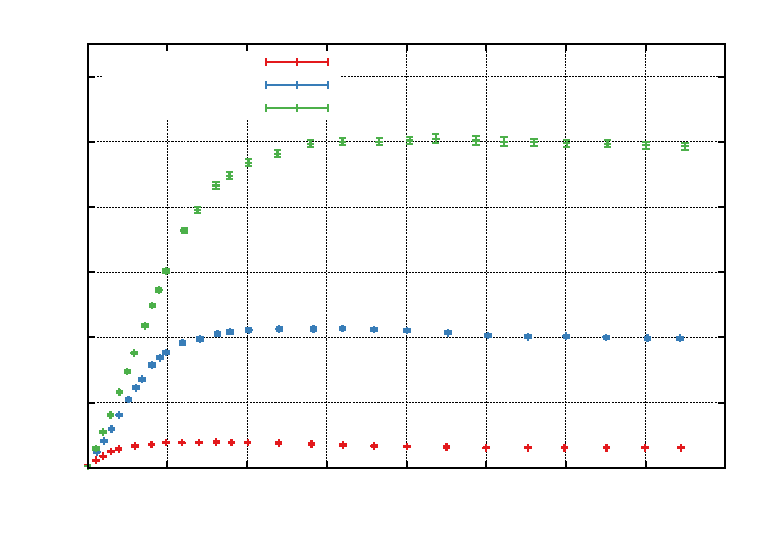
\includegraphics{./plots/kondensatorspannung}}%
    \gplfronttext
  \end{picture}%
\endgroup

	\caption{Abhängigkeit des Ionisationsstroms $I_\mathrm{C}$ von der Kondensatorspannung $U_\mathrm{C}$}
	\label{fig:kondensatorspannung}
\end{figure}

Man sieht sofort, dass sich der Verlauf von Ionisationsstrom in Abhängigkeit der Kondensatorspannung in zwei charakteristische Bereiche einteilen lässt.
Zum einen ist dies der sogenannte Rekombinationsbereich bei kleinen Kondensatorspannungen, in dem das elektrische Feld zwischen den Platten nicht groß genug ist, um alle erzeugten Ionen zu detektieren, da diese aufgrund der geringen Feldstärke rekombinieren können.
Dies äußert sich in dem linearen Anstieg des Ionisationsstroms mit der Kondensatorspannung bis zu einer Grenzspannung bei der die Kurve beginnt in Sättigung zu gehen.
Charakteristisch für diese Grenze ist, dass sie für größere Röhrenspannungen erst bei höheren Kondensatorspannungen eintritt.

Der zweite Bereich ist der Ionisationsbereich, welcher durch das Sättigungsverhalten gekennzeichnet ist.
In diesem ist die Feldstärke so groß, dass fast alle erzeugten Ionen ohne vorige Rekombination zu den Kondensatorplatten gelangen können und folglich als Strom detektiert werden.
Weiterhin lässt sich feststellen, dass das Plateau für höhere Röhrenspannungen größere Ionisationsströme annimmt.
Dies lässt sich dadurch erklären, dass mit wachsender Röhrenspannung das Röntgenspektrum höhere (mittlere) Energie aufweist (vgl. Gleichung \ref{eq:duane_hunt}) und dementsprechend mehr Ionisationsprozesse im Kondensator stattfinden.

Außerhalb unseres Messbereiches ($\SI{0}{V} \leq U_\mathrm{C} \leq \SI{400}{V}$) sind außerdem noch weitere Bereiche zu erwarten.
So kann beispielsweise bei noch höheren Kondensatorspannungen ionisierte Teilchen im elektrischen Feld soviel Energie gewinnen, dass diese weitere Ionen erzeugen, was zu einem verstärkten Ionisationsstrom führt (Proportionalitätsbereich).
Weiterhin kann diese Verstärkung so groß werden, dass die Ionisationsprozesse kaskadieren (Geiger-Bereich).
In Fällen extrem hoher Spannungen kann es zur selbständigen Gasentladung kommen.

Da im Folgenden der Kondensator als Ionisationsdetektor genutzt wird, wird als Betriebsspannung $U_\mathrm{C} = \SI{200}{V}$ gewählt, da sich der Kondensator dort selbst für die maximale Röhrenspannung im Ionisationsbereich befindet.


\subsubsection{Abhängigkeit des Ionisationsstroms vom Emissionsstrom der Röntgenröhre}
\label{sec:abh_emissionsstrom}
Nun wird der Kondensator als Ionisationsdetektor bei einer Spannung $U_\mathrm{C} = \SI{200}{V}$ betrieben, um den Ionisationsstrom in Abhängigkeit des Emissionsstroms $I_\mathrm{E}$ der Röhre zu bestimmen.
Zunächst wird diese mit dem gleichen Versuchsaufbau des vorigen Teils und einer Molybdän-Anode und anschließend mit einer Kupfer-Anode bestimmt.
Dabei wird bei maximaler Röhrenspannung $U = \SI{35}{kV}$ in Emissionsstrom-Schritten von \SI{0.10}{mA} gemessen.
Außerdem ist zu beachten, dass zur Messbereichserweiterung des Elektrometerverstärkers für die Kupferröhre ein Messwiderstand von $R=\SI{100}{\mega\ohm}$ verwendet wurde.
Die Messdaten finden sich in Anhang \ref{app:ionisationsstrom_emissionsstrom} und wurden in Abbildung \ref{fig:abh_emissionsstrom} grafisch dargestellt.
\begin{figure}[hp]
	\centering
	\begin{subfigure}[b]{1\textwidth}
		% GNUPLOT: LaTeX picture with Postscript
\begingroup
  \makeatletter
  \providecommand\color[2][]{%
    \GenericError{(gnuplot) \space\space\space\@spaces}{%
      Package color not loaded in conjunction with
      terminal option `colourtext'%
    }{See the gnuplot documentation for explanation.%
    }{Either use 'blacktext' in gnuplot or load the package
      color.sty in LaTeX.}%
    \renewcommand\color[2][]{}%
  }%
  \providecommand\includegraphics[2][]{%
    \GenericError{(gnuplot) \space\space\space\@spaces}{%
      Package graphicx or graphics not loaded%
    }{See the gnuplot documentation for explanation.%
    }{The gnuplot epslatex terminal needs graphicx.sty or graphics.sty.}%
    \renewcommand\includegraphics[2][]{}%
  }%
  \providecommand\rotatebox[2]{#2}%
  \@ifundefined{ifGPcolor}{%
    \newif\ifGPcolor
    \GPcolortrue
  }{}%
  \@ifundefined{ifGPblacktext}{%
    \newif\ifGPblacktext
    \GPblacktexttrue
  }{}%
  % define a \g@addto@macro without @ in the name:
  \let\gplgaddtomacro\g@addto@macro
  % define empty templates for all commands taking text:
  \gdef\gplbacktext{}%
  \gdef\gplfronttext{}%
  \makeatother
  \ifGPblacktext
    % no textcolor at all
    \def\colorrgb#1{}%
    \def\colorgray#1{}%
  \else
    % gray or color?
    \ifGPcolor
      \def\colorrgb#1{\color[rgb]{#1}}%
      \def\colorgray#1{\color[gray]{#1}}%
      \expandafter\def\csname LTw\endcsname{\color{white}}%
      \expandafter\def\csname LTb\endcsname{\color{black}}%
      \expandafter\def\csname LTa\endcsname{\color{black}}%
      \expandafter\def\csname LT0\endcsname{\color[rgb]{1,0,0}}%
      \expandafter\def\csname LT1\endcsname{\color[rgb]{0,1,0}}%
      \expandafter\def\csname LT2\endcsname{\color[rgb]{0,0,1}}%
      \expandafter\def\csname LT3\endcsname{\color[rgb]{1,0,1}}%
      \expandafter\def\csname LT4\endcsname{\color[rgb]{0,1,1}}%
      \expandafter\def\csname LT5\endcsname{\color[rgb]{1,1,0}}%
      \expandafter\def\csname LT6\endcsname{\color[rgb]{0,0,0}}%
      \expandafter\def\csname LT7\endcsname{\color[rgb]{1,0.3,0}}%
      \expandafter\def\csname LT8\endcsname{\color[rgb]{0.5,0.5,0.5}}%
    \else
      % gray
      \def\colorrgb#1{\color{black}}%
      \def\colorgray#1{\color[gray]{#1}}%
      \expandafter\def\csname LTw\endcsname{\color{white}}%
      \expandafter\def\csname LTb\endcsname{\color{black}}%
      \expandafter\def\csname LTa\endcsname{\color{black}}%
      \expandafter\def\csname LT0\endcsname{\color{black}}%
      \expandafter\def\csname LT1\endcsname{\color{black}}%
      \expandafter\def\csname LT2\endcsname{\color{black}}%
      \expandafter\def\csname LT3\endcsname{\color{black}}%
      \expandafter\def\csname LT4\endcsname{\color{black}}%
      \expandafter\def\csname LT5\endcsname{\color{black}}%
      \expandafter\def\csname LT6\endcsname{\color{black}}%
      \expandafter\def\csname LT7\endcsname{\color{black}}%
      \expandafter\def\csname LT8\endcsname{\color{black}}%
    \fi
  \fi
    \setlength{\unitlength}{0.0500bp}%
    \ifx\gptboxheight\undefined%
      \newlength{\gptboxheight}%
      \newlength{\gptboxwidth}%
      \newsavebox{\gptboxtext}%
    \fi%
    \setlength{\fboxrule}{0.5pt}%
    \setlength{\fboxsep}{1pt}%
\begin{picture}(7200.00,5040.00)%
    \gplgaddtomacro\gplbacktext{%
      \csname LTb\endcsname%
      \put(550,704){\makebox(0,0)[r]{\strut{}$0$}}%
      \csname LTb\endcsname%
      \put(550,1383){\makebox(0,0)[r]{\strut{}$1$}}%
      \csname LTb\endcsname%
      \put(550,2061){\makebox(0,0)[r]{\strut{}$2$}}%
      \csname LTb\endcsname%
      \put(550,2740){\makebox(0,0)[r]{\strut{}$3$}}%
      \csname LTb\endcsname%
      \put(550,3418){\makebox(0,0)[r]{\strut{}$4$}}%
      \csname LTb\endcsname%
      \put(550,4097){\makebox(0,0)[r]{\strut{}$5$}}%
      \csname LTb\endcsname%
      \put(550,4775){\makebox(0,0)[r]{\strut{}$6$}}%
      \csname LTb\endcsname%
      \put(682,484){\makebox(0,0){\strut{}$0$}}%
      \csname LTb\endcsname%
      \put(1906,484){\makebox(0,0){\strut{}$0{,}2$}}%
      \csname LTb\endcsname%
      \put(3130,484){\makebox(0,0){\strut{}$0{,}4$}}%
      \csname LTb\endcsname%
      \put(4355,484){\makebox(0,0){\strut{}$0{,}6$}}%
      \csname LTb\endcsname%
      \put(5579,484){\makebox(0,0){\strut{}$0{,}8$}}%
      \csname LTb\endcsname%
      \put(6803,484){\makebox(0,0){\strut{}$1$}}%
    }%
    \gplgaddtomacro\gplfronttext{%
      \csname LTb\endcsname%
      \put(176,2739){\rotatebox{-270}{\makebox(0,0){\strut{}Ionisationsstrom $I_\mathrm{C} / \si{nA}$}}}%
      \put(3742,154){\makebox(0,0){\strut{}Emissionsstrom $I_\mathrm{E} / \si{mA}$}}%
      \csname LTb\endcsname%
      \put(2002,4602){\makebox(0,0)[r]{\strut{}Messdaten}}%
      \csname LTb\endcsname%
      \put(2002,4382){\makebox(0,0)[r]{\strut{}Anpassung}}%
    }%
    \gplbacktext
    \put(0,0){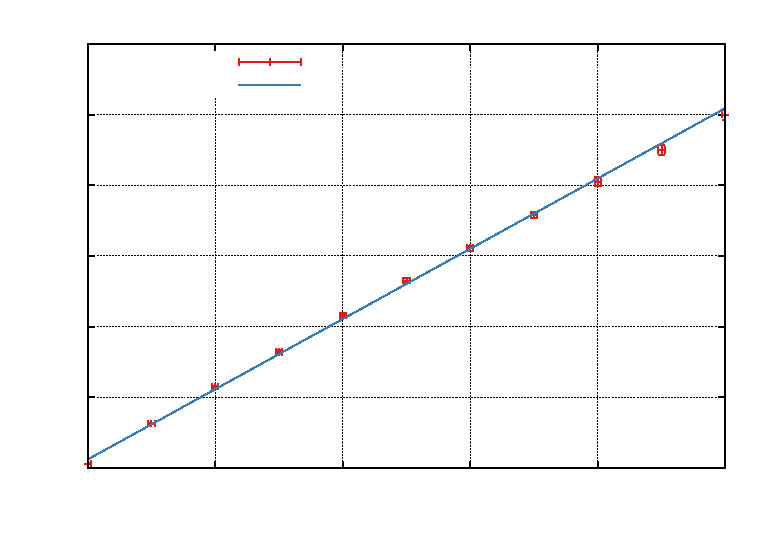
\includegraphics{./plots/abh_emissionsstrom/mo}}%
    \gplfronttext
  \end{picture}%
\endgroup

		\subcaption{Molybdän-Röhre mit Anpassung einer linearen Funktion}
		\label{fig:mo_emissionsstrom}
	\end{subfigure}
	
	\vspace{10mm}
	
	\begin{subfigure}[b]{1\textwidth}
		\begin{tabular}{SSSSSS}
	\toprule
	{$U / \si{kV}$} & {$\Delta U / \si{kV}$} & {$U_{I_\mathrm{C}} / \si{mV}$} & {$\Delta U_{I_\mathrm{C}} / \si{mV}$} & {$I_\mathrm{C} / \si{nA}$} & {$\Delta I_\mathrm{C} / \si{nA}$} \\ \midrule
	0.00   & 0.05      & 13        & 2            & 0.13      & 0.03         \\
	2.50   & 0.05      & 13        & 2            & 0.13      & 0.03         \\
	5.00   & 0.05      & 38        & 2            & 0.38      & 0.03         \\
	7.50   & 0.05      & 180       & 5            & 1.80      & 0.06         \\
	10.00  & 0.05      & 550       & 10           & 5.50      & 0.12         \\
	12.50  & 0.05      & 1090      & 10           & 10.90     & 0.15         \\
	15.00  & 0.05      & 1700      & 10           & 17.00     & 0.20         \\
	17.50  & 0.05      & 2330      & 10           & 23.30     & 0.26         \\
	20.00  & 0.05      & 2960      & 10           & 29.60     & 0.32         \\
	22.50  & 0.05      & 3510      & 10           & 35.10     & 0.37         \\
	25.00  & 0.05      & 3990      & 10           & 39.90     & 0.42         \\
	27.50  & 0.05      & 4390      & 10           & 43.90     & 0.46         \\
	30.00  & 0.05      & 4730      & 10           & 47.30     & 0.49         \\
	32.50  & 0.05      & 5020      & 10           & 50.20     & 0.52         \\
	35.00  & 0.05      & 5260      & 20           & 52.60     & 0.57         \\ \bottomrule
\end{tabular}
		\subcaption{Kupfer-Röhre mit starker Abweichung vom erwarteten linearen Verhalten}
		\label{fig:cu_emissionsstrom}
	\end{subfigure}
	\caption{Abhängigkeit des Ionisationsstroms $I_\mathrm{C}$ vom Emissionsstrom $I_\mathrm{E}$ für verschiedene Röntgenröhren. Beide Messungen wurden bei maximaler Röhrenspannung $U=\SI{35}{kV}$ durchgeführt.}
	\label{fig:abh_emissionsstrom}
\end{figure}
Eine Erhöhung des Emissionsstroms führt zu einer proportionalen Anstieg der Anzahl der Elektronen, die in einem Zeitintervall aus der Röhrenkathode austreten.
Dadurch erhöht sich dementsprechend die Intensität der Röntgenstrahlung um denselben Faktor, da jedes der emittierten Elektronen (unabhängig von deren Anzahl, sofern Raumladungseffekte vernachlässigt werden können) mit dem Anodenmaterial interagiert.
Somit steigt die Intensität der Röntgenstrahlung, wobei das Spektrum selbst unverändert bleibt, da die Beschleunigungsspannung gleich bleibt.
Darüber hinaus führt eine Intensitätserhöhung zu einem proportionalen Anstieg der Ionisationen zwischen den Kondensatorplatten, was dann zu einer ebenso proportionalen Erhöhung des Ionisationsstroms führt.
Diese Tatsache ist für die Molybdän-Röhre in Abbildung \ref{fig:mo_emissionsstrom} gut zu beobachten.
An diese wurde die Anpassung einer Geraden:
\begin{align}
	I_\mathrm{C} = \lambda \cdot I_\mathrm{E} + I_0
\end{align}
durchgeführt, wobei entgegen der erwarteten Ursprungsgerade ein Achsenabschnitt $I_0$ verwendet wird, welcher im Spannungsoffset des Elektrometerverstärkers begründet liegt.
\begin{align*}
	\lambda &= \num{4.970 +- 0.055e-6}\\
	I_0 &= \SI{0.120 +- 0.022}{nA}
\end{align*}
Für die Kupferröhre in Abbildung \ref{fig:cu_emissionsstrom} ist eine starke Abweichung von dem linearen Zusammenhang sichtbar.
Eine mögliche Ursache dafür könnte die höhere Intensität der emittierten Röntgenstrahlung sein, welche im Kondensator so viele Ionisationen durchführt, dass die zwischen den Kondensatorplatten entstehende Raumladung zu einer Sättigung führt.


\subsubsection{Abhängigkeit des Ionisationsstroms von der Röhrenspannung}
\label{sec:abh_roehrenspannung}
Analog zum vorigen Abschnitt soll nun die Abhängigkeit des Ionisationsstroms $I_\mathrm{C}$ von der Röhrenspannung $U$ für Molybdän- und Kupferröhre untersucht werden.
Dabei wird beim maximalen Emissionsstrom $I_\mathrm{E} = \SI{1.00}{mA}$ die Röhrenspannung in Schritten von \SI{2.5}{kV} von \SI{0}{kV} bis \SI{35}{kV} variiert und der Ionisationsstrom mithilfe des Elektrometerverstärkers gemessen.
Der Fehler der Röhrenspannung wird anhand der letzten Stelle der Digitalanzeige des Röntgengerätes auf $\Delta U = \SI{0.05}{kV}$ abgeschätzt.
Die aufgenommenen Messdaten wurden im Anhang \ref{app:ionisationsstrom_roehrenspannung} aufgetragen und in Abbildung \ref{fig:abh_roehrenspannung} grafisch dargestellt.
\begin{figure}[hp]
	\centering
	\vspace{-10mm}
	
	\begin{subfigure}[b]{1\textwidth}
		% GNUPLOT: LaTeX picture with Postscript
\begingroup
  \makeatletter
  \providecommand\color[2][]{%
    \GenericError{(gnuplot) \space\space\space\@spaces}{%
      Package color not loaded in conjunction with
      terminal option `colourtext'%
    }{See the gnuplot documentation for explanation.%
    }{Either use 'blacktext' in gnuplot or load the package
      color.sty in LaTeX.}%
    \renewcommand\color[2][]{}%
  }%
  \providecommand\includegraphics[2][]{%
    \GenericError{(gnuplot) \space\space\space\@spaces}{%
      Package graphicx or graphics not loaded%
    }{See the gnuplot documentation for explanation.%
    }{The gnuplot epslatex terminal needs graphicx.sty or graphics.sty.}%
    \renewcommand\includegraphics[2][]{}%
  }%
  \providecommand\rotatebox[2]{#2}%
  \@ifundefined{ifGPcolor}{%
    \newif\ifGPcolor
    \GPcolortrue
  }{}%
  \@ifundefined{ifGPblacktext}{%
    \newif\ifGPblacktext
    \GPblacktexttrue
  }{}%
  % define a \g@addto@macro without @ in the name:
  \let\gplgaddtomacro\g@addto@macro
  % define empty templates for all commands taking text:
  \gdef\gplbacktext{}%
  \gdef\gplfronttext{}%
  \makeatother
  \ifGPblacktext
    % no textcolor at all
    \def\colorrgb#1{}%
    \def\colorgray#1{}%
  \else
    % gray or color?
    \ifGPcolor
      \def\colorrgb#1{\color[rgb]{#1}}%
      \def\colorgray#1{\color[gray]{#1}}%
      \expandafter\def\csname LTw\endcsname{\color{white}}%
      \expandafter\def\csname LTb\endcsname{\color{black}}%
      \expandafter\def\csname LTa\endcsname{\color{black}}%
      \expandafter\def\csname LT0\endcsname{\color[rgb]{1,0,0}}%
      \expandafter\def\csname LT1\endcsname{\color[rgb]{0,1,0}}%
      \expandafter\def\csname LT2\endcsname{\color[rgb]{0,0,1}}%
      \expandafter\def\csname LT3\endcsname{\color[rgb]{1,0,1}}%
      \expandafter\def\csname LT4\endcsname{\color[rgb]{0,1,1}}%
      \expandafter\def\csname LT5\endcsname{\color[rgb]{1,1,0}}%
      \expandafter\def\csname LT6\endcsname{\color[rgb]{0,0,0}}%
      \expandafter\def\csname LT7\endcsname{\color[rgb]{1,0.3,0}}%
      \expandafter\def\csname LT8\endcsname{\color[rgb]{0.5,0.5,0.5}}%
    \else
      % gray
      \def\colorrgb#1{\color{black}}%
      \def\colorgray#1{\color[gray]{#1}}%
      \expandafter\def\csname LTw\endcsname{\color{white}}%
      \expandafter\def\csname LTb\endcsname{\color{black}}%
      \expandafter\def\csname LTa\endcsname{\color{black}}%
      \expandafter\def\csname LT0\endcsname{\color{black}}%
      \expandafter\def\csname LT1\endcsname{\color{black}}%
      \expandafter\def\csname LT2\endcsname{\color{black}}%
      \expandafter\def\csname LT3\endcsname{\color{black}}%
      \expandafter\def\csname LT4\endcsname{\color{black}}%
      \expandafter\def\csname LT5\endcsname{\color{black}}%
      \expandafter\def\csname LT6\endcsname{\color{black}}%
      \expandafter\def\csname LT7\endcsname{\color{black}}%
      \expandafter\def\csname LT8\endcsname{\color{black}}%
    \fi
  \fi
    \setlength{\unitlength}{0.0500bp}%
    \ifx\gptboxheight\undefined%
      \newlength{\gptboxheight}%
      \newlength{\gptboxwidth}%
      \newsavebox{\gptboxtext}%
    \fi%
    \setlength{\fboxrule}{0.5pt}%
    \setlength{\fboxsep}{1pt}%
\begin{picture}(7200.00,5040.00)%
    \gplgaddtomacro\gplbacktext{%
      \csname LTb\endcsname%
      \put(550,704){\makebox(0,0)[r]{\strut{}$0$}}%
      \csname LTb\endcsname%
      \put(550,1383){\makebox(0,0)[r]{\strut{}$1$}}%
      \csname LTb\endcsname%
      \put(550,2061){\makebox(0,0)[r]{\strut{}$2$}}%
      \csname LTb\endcsname%
      \put(550,2740){\makebox(0,0)[r]{\strut{}$3$}}%
      \csname LTb\endcsname%
      \put(550,3418){\makebox(0,0)[r]{\strut{}$4$}}%
      \csname LTb\endcsname%
      \put(550,4097){\makebox(0,0)[r]{\strut{}$5$}}%
      \csname LTb\endcsname%
      \put(550,4775){\makebox(0,0)[r]{\strut{}$6$}}%
      \csname LTb\endcsname%
      \put(682,484){\makebox(0,0){\strut{}$0$}}%
      \csname LTb\endcsname%
      \put(1906,484){\makebox(0,0){\strut{}$0{,}2$}}%
      \csname LTb\endcsname%
      \put(3130,484){\makebox(0,0){\strut{}$0{,}4$}}%
      \csname LTb\endcsname%
      \put(4355,484){\makebox(0,0){\strut{}$0{,}6$}}%
      \csname LTb\endcsname%
      \put(5579,484){\makebox(0,0){\strut{}$0{,}8$}}%
      \csname LTb\endcsname%
      \put(6803,484){\makebox(0,0){\strut{}$1$}}%
    }%
    \gplgaddtomacro\gplfronttext{%
      \csname LTb\endcsname%
      \put(176,2739){\rotatebox{-270}{\makebox(0,0){\strut{}Ionisationsstrom $I_\mathrm{C} / \si{nA}$}}}%
      \put(3742,154){\makebox(0,0){\strut{}Emissionsstrom $I_\mathrm{E} / \si{mA}$}}%
      \csname LTb\endcsname%
      \put(2002,4602){\makebox(0,0)[r]{\strut{}Messdaten}}%
      \csname LTb\endcsname%
      \put(2002,4382){\makebox(0,0)[r]{\strut{}Anpassung}}%
    }%
    \gplbacktext
    \put(0,0){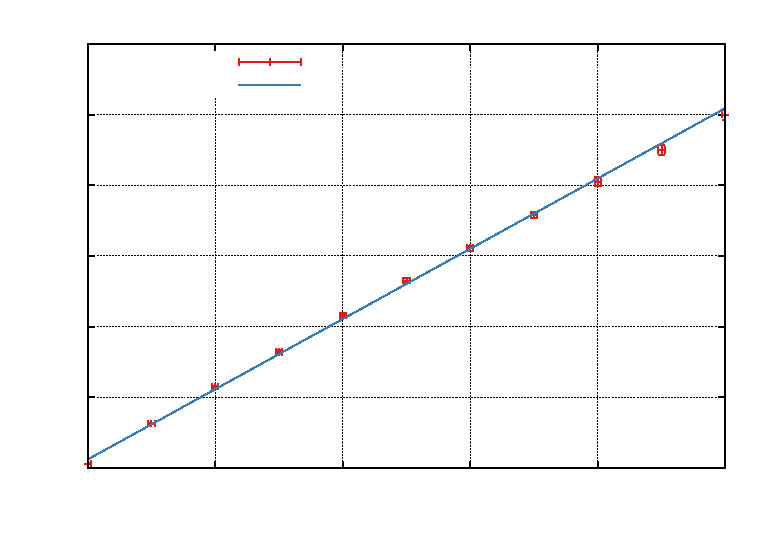
\includegraphics{./plots/abh_emissionsstrom/mo}}%
    \gplfronttext
  \end{picture}%
\endgroup

		\subcaption{Molybdän-Röhre mit charakteristischen Linien $\mathrm{K}_\alpha$ (\SI{17.4}{keV}) und $\mathrm{K}_\beta$ (\SI{19.6}{keV}) \cite{booklet}}
		\label{fig:mo_roehrenspannung}
	\end{subfigure}
	
	\vspace{2.5mm}
	
	\begin{subfigure}[b]{1\textwidth}
		\begin{tabular}{SSSSSS}
	\toprule
	{$U / \si{kV}$} & {$\Delta U / \si{kV}$} & {$U_{I_\mathrm{C}} / \si{mV}$} & {$\Delta U_{I_\mathrm{C}} / \si{mV}$} & {$I_\mathrm{C} / \si{nA}$} & {$\Delta I_\mathrm{C} / \si{nA}$} \\ \midrule
	0.00   & 0.05      & 13        & 2            & 0.13      & 0.03         \\
	2.50   & 0.05      & 13        & 2            & 0.13      & 0.03         \\
	5.00   & 0.05      & 38        & 2            & 0.38      & 0.03         \\
	7.50   & 0.05      & 180       & 5            & 1.80      & 0.06         \\
	10.00  & 0.05      & 550       & 10           & 5.50      & 0.12         \\
	12.50  & 0.05      & 1090      & 10           & 10.90     & 0.15         \\
	15.00  & 0.05      & 1700      & 10           & 17.00     & 0.20         \\
	17.50  & 0.05      & 2330      & 10           & 23.30     & 0.26         \\
	20.00  & 0.05      & 2960      & 10           & 29.60     & 0.32         \\
	22.50  & 0.05      & 3510      & 10           & 35.10     & 0.37         \\
	25.00  & 0.05      & 3990      & 10           & 39.90     & 0.42         \\
	27.50  & 0.05      & 4390      & 10           & 43.90     & 0.46         \\
	30.00  & 0.05      & 4730      & 10           & 47.30     & 0.49         \\
	32.50  & 0.05      & 5020      & 10           & 50.20     & 0.52         \\
	35.00  & 0.05      & 5260      & 20           & 52.60     & 0.57         \\ \bottomrule
\end{tabular}
		\subcaption{Kupfer-Röhre mit charakteristischen Linien $\mathrm{K}_\alpha$ (\SI{8.04}{keV}) und $\mathrm{K}_\beta$ (\SI{8.91}{keV}) \cite{booklet}}
		\label{fig:cu_roehrenspannung}
	\end{subfigure}
	\caption{Abhängigkeit des Ionisationsstroms $I_\mathrm{C}$ von der Röhrenspannung $U$ für verschiedene Röntgenröhren. Beide Messungen wurden bei maximalem Emissionsstrom $I_\mathrm{E} = \SI{1.00}{mA}$ durchgeführt.}
	\label{fig:abh_roehrenspannung}
\end{figure}

Im Gegensatz zur Variation des Emissionsstroms kann hier kein lineares Verhältnis zwischen Ionisationsstrom und Röhrenspannung beobachtet werden.
Dies liegt zum einen daran, dass die mittlere Energie des kontinuierlichen Bremsstrahlungsspektrums nicht proportional zur Röhrenspannung ist und darüber hinaus daran, dass die charakteristischen Linien der Anode eine signifikante Auswirkung auf das resultierende Spektrum haben.
Generell wird aber eine Zunahme des Ionisationsstroms erwartet, da der Anstieg der mittleren Energie des Röntgenspektrums zur Zunahme der Anzahl von Ionisationen zwischen den Kondensatorplatten führt.
Die minimalen Beschleunigungsspannungen (Duane-Hunt-Gesetz) zur Anregung der wichtigsten charakteristischen Linien der jeweiligen Anode wurden in Abbildung \ref{fig:abh_roehrenspannung} markiert und fallen mit dem starken Anstieg des Ionisationsstroms zusammen.
Weiterhin ist für die Kupfer-Röhre in Abbildung \ref{fig:cu_roehrenspannung} erneut ein Abflachen des Ionisationsstroms bei hohen Röhrenspannungen zu beobachten, was erneut auf Raumladungseffekte zurückzuführen sein könnte.


\subsubsection{Bestimmung der Ionendosisleistung im Kondensator}
Zur Bestimmung der Ionendosisleistung im Raum zwischen den Kondensatorplatten, muss gemäß Abschnitt \ref{sec:ionendosis} die Masse des durchstrahlten Volumens berechnet werden.
Dies geschieht indem durch geometrische Betrachtungen das durchstrahlte Volumen im Kondensator berechnet wird und anschließend anhand der gemessenen Temperatur $T$ und Luftdruck $p$ die Dichte der Luft $\rho$ im Experimentierraum berechnet wird.\\
\\
\textbf{Berechnung des durchstrahlten Volumens:}\\
\begin{figure}[h]
	\centering
	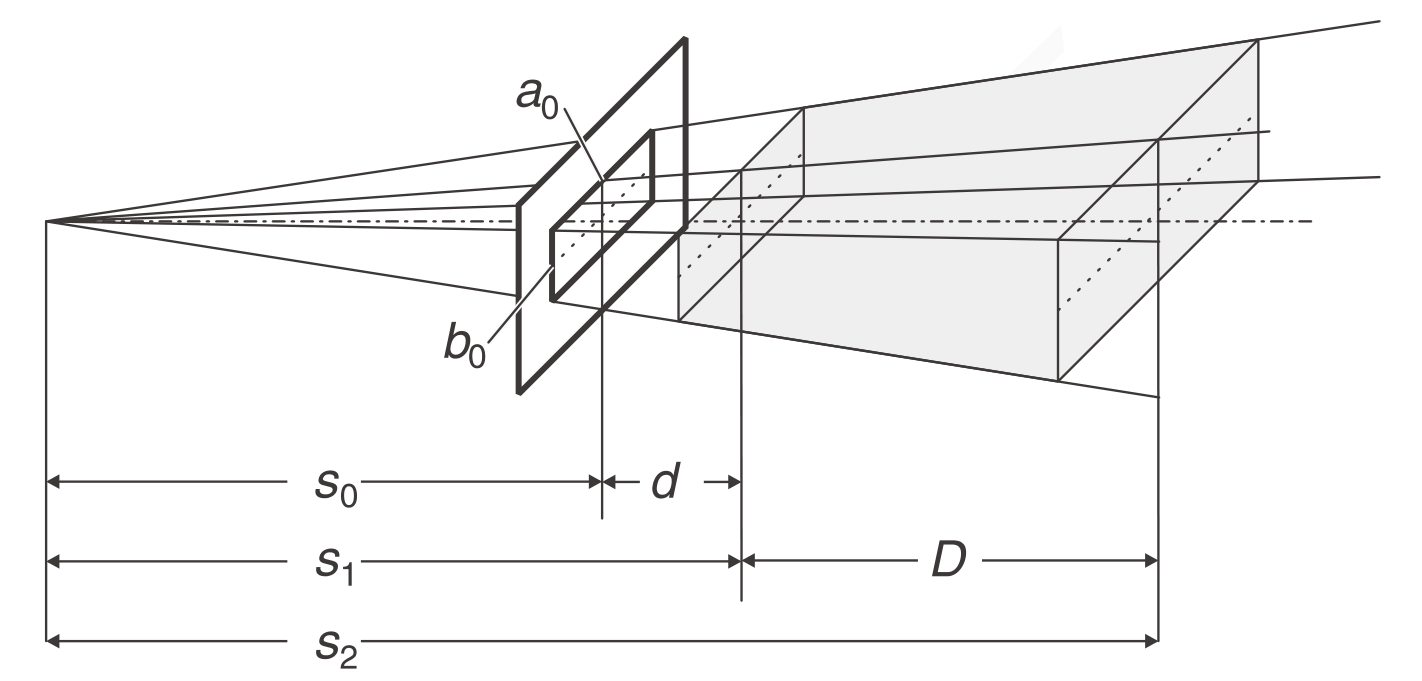
\includegraphics[width=0.8\textwidth]{./figures/volumen_kondensator.png}
	\caption{Geometrie des durchstrahlten Volumens im Plattenkondensator \cite{ld_didactic}. Die näherungsweise punktförmige Röntgenquelle wird durch eine Rechteckblende der Fläche $A_0 = a_0 \cdot b_0$ begrenzt. In einer Entfernung $d$ von der Blende befindet sich der Plattenkondensator mit Länge $D$.}
	\label{fig:kondensator_volumen}
\end{figure}
Das Volumen des Pyramidenstumpfs in Abbildung \ref{fig:kondensator_volumen} kann einfach durch Integration über die Schnittfläche $A(s)$ im Abstand $s$ von der Röntgenquelle berechnet werden:
\begin{align}
	V = \int_{s_1}^{s_2} A(s) \, \mathrm{d}s
\end{align}
Da die Abstände der einzelnen Komponenten von der Quelle bekannt sind, kann über die bekannten Blendenmaße und dem Strahlensatz die Kantenlängen der Schnittfläche durch:
\begin{align}
	a(s) = \frac{a_0}{s_0} \cdot s \qquad b(s) = \frac{b_0}{s_0} \cdot s
\end{align}
berechnet werden.
Dann ergibt sich für die Schnittfläche:
\begin{align}
	A(s) = a(s) \cdot b(s) = \frac{a_0 \, b_0}{s_0^2} \cdot s^2
\end{align}
Die Durchführung der Integration liefert folglich:
\begin{align}
	V &= \frac{1}{3} \, \frac{a_0 \, b_0}{s_0^2} \left[ s_2^3 - s_1^3 \right] \nonumber\\
	  &= \frac{1}{3} \, \frac{a_0 \, b_0}{s_0^2} \left[ (s_0 + d + D)^3 - (s_0 + d)^3 \right]
	  \label{eq:volumen_kondensator}
\end{align}
wobei im letzten Schritt die bekannten Größen substituiert wurden.
Mit den in \cite{anleitung} aufgeführten Maßen:
\begin{align*}
	a_0 &= \SI{4.50 +- 0.05}{cm} \qquad b_0 = \SI{0.6 +- 0.05}{cm}\\
	d &= \SI{2.5 +- 0.05}{cm} \qquad D = \SI{16.00 +- 0.05}{cm}\\
	s_0 &= \SI{15.50 +- 0.05}{cm}
\end{align*}
Dabei wurde der Fehler der einzelnen Maße anhand der in \cite{anleitung} angegeben Stellen abgeschätzt.
Mit dem Volumen aus Gleichung \eqref{eq:volumen_kondensator} und der Gauß'schen Fehlerfortpflanzung folgt:
\begin{align}
	V = \SI{125 +- 11}{\centi\meter\cubed}
\end{align}
dabei soll aus Übersichtsgründen auf eine explizite Angabe der Formel verzichtet werden.\\
\\
\textbf{Dichte der Luft im Experimentierraum:}\\
Die Dichte der Luft kann mit der idealen Gasgleichung aus Luftdruck und Temperatur im Versuchsraum berechnet werden.
Diese wurden an einem Thermometer/Barometer abgelesen:
\begin{align}
	T &= \SI{24.5 +- 1.5}{\degreeCelsius} \\
	p &= \SI{993 +- 3}{hPa}
\end{align}
dabei wurden die Messgenauigkeiten in \cite{anleitung} gegeben.
Mit der idealen Gasgleichung folgt dann:
\begin{align*}
	\frac{p \, V}{T} = \mathrm{const}
\end{align*}
was unter den Normalbedingungen ($p_0 = \SI{1013}{hPa}$, $T_0 = \SI{273}{K}$ und $\rho_0 = \SI{1.293}{\kilogram\per\metre\cubed}$) auf:
\begin{align*}
	\frac{p_0 \, V_0}{T_0} = \frac{p \, V}{T}
\end{align*}
führt.
Division beider Seiten durch $\rho = \frac{M}{V}$ und Auflösen nach $\rho$ führt zu:
\begin{align}
	\rho = \rho_0 \cdot \frac{T_0}{T} \cdot \frac{p}{p_0}
\end{align}
Der Fehler ist erneut durch Gauß'sche Fehlerfortpflanzung gegeben durch:
\begin{align}
	\Delta \rho = \rho \, \sqrt{ \left( \frac{\Delta T}{T} \right)^2 + \left( \frac{\Delta p}{p} \right)^2}
\end{align}
Mit den oben erwähnten Messwerten ergibt sich für die Dichte der Luft zum Zeitpunkt der Versuchsdurchführung:
\begin{align}
	\rho = \SI{1.1625 +- 0.0069}{\kilogram\per\metre\cubed}
\end{align}\\
\\
\textbf{Berechnung der Gesamtmasse des durchstrahlten Volumens:}\\
Die Gesamtmasse kann nun einfach als Produkt von Dichte $\rho$ und Volumen $V$ berechnet werden:
\begin{align}
	m = \rho \cdot V \qquad \Delta m = \sqrt{V^2 \cdot \Delta \rho^2 + \rho^2 \cdot \Delta V^2}
\end{align}
Mit den obigen Werten ergibt sich:
\begin{align}
	m = \SI{1.45 +- 0.13e-4}{kg}
\end{align}\\
Da nun die Masse des durchstrahlten Volumens berechnet ist, kann die mittlere Ionendosisleistungen $\braket{j}$ aus den Messungen des Ionisationsstroms der vorigen Aufgabenteile berechnet werden.
Die konkrete Berechung erfolgt durch:
\begin{align}
	\braket{j} = \frac{I_\mathrm{C}}{m} \qquad \Delta \braket{j} = \braket{j} \cdot \sqrt{\frac{\Delta I_\mathrm{C}^2}{I_\mathrm{C}^2} + \frac{\Delta m^2}{m^2}}
	\label{eq:fehler_dosisleistung}
\end{align}
Der Umrechnungsfaktor:
\begin{align*}
	\SI{1}{\micro\ampere\per\kilogram} = \SI{32.4}{\micro\sievert\per\second} = \SI{0.11664}{\sievert\per\hour}
\end{align*}
ermöglicht die Umrechnung der mittleren Ionendosisleistung $\braket{j}$ in die Äquivalentdosisleistung $\dot{H}$.
Zur Berechnung der Ionendosisleistung die Messwerte der vorigen Aufgabenteile verwendet, welche in Anhang \ref{app:ionisationsstrom_emissionsstrom} und \ref{app:ionisationsstrom_roehrenspannung} tabelliert sind.
Die grafische Darstellung der Dosisleistungen wurde in den Abbildungen \ref{fig:dosis_emissionsstrom} und \ref{fig:dosis_roehrenspannung} durchgeführt.
\begin{figure}[hp]
	\begin{subfigure}[b]{\textwidth}
		\centering
		% GNUPLOT: LaTeX picture with Postscript
\begingroup
  \makeatletter
  \providecommand\color[2][]{%
    \GenericError{(gnuplot) \space\space\space\@spaces}{%
      Package color not loaded in conjunction with
      terminal option `colourtext'%
    }{See the gnuplot documentation for explanation.%
    }{Either use 'blacktext' in gnuplot or load the package
      color.sty in LaTeX.}%
    \renewcommand\color[2][]{}%
  }%
  \providecommand\includegraphics[2][]{%
    \GenericError{(gnuplot) \space\space\space\@spaces}{%
      Package graphicx or graphics not loaded%
    }{See the gnuplot documentation for explanation.%
    }{The gnuplot epslatex terminal needs graphicx.sty or graphics.sty.}%
    \renewcommand\includegraphics[2][]{}%
  }%
  \providecommand\rotatebox[2]{#2}%
  \@ifundefined{ifGPcolor}{%
    \newif\ifGPcolor
    \GPcolortrue
  }{}%
  \@ifundefined{ifGPblacktext}{%
    \newif\ifGPblacktext
    \GPblacktexttrue
  }{}%
  % define a \g@addto@macro without @ in the name:
  \let\gplgaddtomacro\g@addto@macro
  % define empty templates for all commands taking text:
  \gdef\gplbacktext{}%
  \gdef\gplfronttext{}%
  \makeatother
  \ifGPblacktext
    % no textcolor at all
    \def\colorrgb#1{}%
    \def\colorgray#1{}%
  \else
    % gray or color?
    \ifGPcolor
      \def\colorrgb#1{\color[rgb]{#1}}%
      \def\colorgray#1{\color[gray]{#1}}%
      \expandafter\def\csname LTw\endcsname{\color{white}}%
      \expandafter\def\csname LTb\endcsname{\color{black}}%
      \expandafter\def\csname LTa\endcsname{\color{black}}%
      \expandafter\def\csname LT0\endcsname{\color[rgb]{1,0,0}}%
      \expandafter\def\csname LT1\endcsname{\color[rgb]{0,1,0}}%
      \expandafter\def\csname LT2\endcsname{\color[rgb]{0,0,1}}%
      \expandafter\def\csname LT3\endcsname{\color[rgb]{1,0,1}}%
      \expandafter\def\csname LT4\endcsname{\color[rgb]{0,1,1}}%
      \expandafter\def\csname LT5\endcsname{\color[rgb]{1,1,0}}%
      \expandafter\def\csname LT6\endcsname{\color[rgb]{0,0,0}}%
      \expandafter\def\csname LT7\endcsname{\color[rgb]{1,0.3,0}}%
      \expandafter\def\csname LT8\endcsname{\color[rgb]{0.5,0.5,0.5}}%
    \else
      % gray
      \def\colorrgb#1{\color{black}}%
      \def\colorgray#1{\color[gray]{#1}}%
      \expandafter\def\csname LTw\endcsname{\color{white}}%
      \expandafter\def\csname LTb\endcsname{\color{black}}%
      \expandafter\def\csname LTa\endcsname{\color{black}}%
      \expandafter\def\csname LT0\endcsname{\color{black}}%
      \expandafter\def\csname LT1\endcsname{\color{black}}%
      \expandafter\def\csname LT2\endcsname{\color{black}}%
      \expandafter\def\csname LT3\endcsname{\color{black}}%
      \expandafter\def\csname LT4\endcsname{\color{black}}%
      \expandafter\def\csname LT5\endcsname{\color{black}}%
      \expandafter\def\csname LT6\endcsname{\color{black}}%
      \expandafter\def\csname LT7\endcsname{\color{black}}%
      \expandafter\def\csname LT8\endcsname{\color{black}}%
    \fi
  \fi
    \setlength{\unitlength}{0.0500bp}%
    \ifx\gptboxheight\undefined%
      \newlength{\gptboxheight}%
      \newlength{\gptboxwidth}%
      \newsavebox{\gptboxtext}%
    \fi%
    \setlength{\fboxrule}{0.5pt}%
    \setlength{\fboxsep}{1pt}%
\begin{picture}(7200.00,5040.00)%
    \gplgaddtomacro\gplbacktext{%
      \csname LTb\endcsname%
      \put(550,704){\makebox(0,0)[r]{\strut{}$0$}}%
      \csname LTb\endcsname%
      \put(550,1383){\makebox(0,0)[r]{\strut{}$1$}}%
      \csname LTb\endcsname%
      \put(550,2061){\makebox(0,0)[r]{\strut{}$2$}}%
      \csname LTb\endcsname%
      \put(550,2740){\makebox(0,0)[r]{\strut{}$3$}}%
      \csname LTb\endcsname%
      \put(550,3418){\makebox(0,0)[r]{\strut{}$4$}}%
      \csname LTb\endcsname%
      \put(550,4097){\makebox(0,0)[r]{\strut{}$5$}}%
      \csname LTb\endcsname%
      \put(550,4775){\makebox(0,0)[r]{\strut{}$6$}}%
      \csname LTb\endcsname%
      \put(682,484){\makebox(0,0){\strut{}$0$}}%
      \csname LTb\endcsname%
      \put(1906,484){\makebox(0,0){\strut{}$0{,}2$}}%
      \csname LTb\endcsname%
      \put(3130,484){\makebox(0,0){\strut{}$0{,}4$}}%
      \csname LTb\endcsname%
      \put(4355,484){\makebox(0,0){\strut{}$0{,}6$}}%
      \csname LTb\endcsname%
      \put(5579,484){\makebox(0,0){\strut{}$0{,}8$}}%
      \csname LTb\endcsname%
      \put(6803,484){\makebox(0,0){\strut{}$1$}}%
    }%
    \gplgaddtomacro\gplfronttext{%
      \csname LTb\endcsname%
      \put(176,2739){\rotatebox{-270}{\makebox(0,0){\strut{}Ionisationsstrom $I_\mathrm{C} / \si{nA}$}}}%
      \put(3742,154){\makebox(0,0){\strut{}Emissionsstrom $I_\mathrm{E} / \si{mA}$}}%
      \csname LTb\endcsname%
      \put(2002,4602){\makebox(0,0)[r]{\strut{}Messdaten}}%
      \csname LTb\endcsname%
      \put(2002,4382){\makebox(0,0)[r]{\strut{}Anpassung}}%
    }%
    \gplbacktext
    \put(0,0){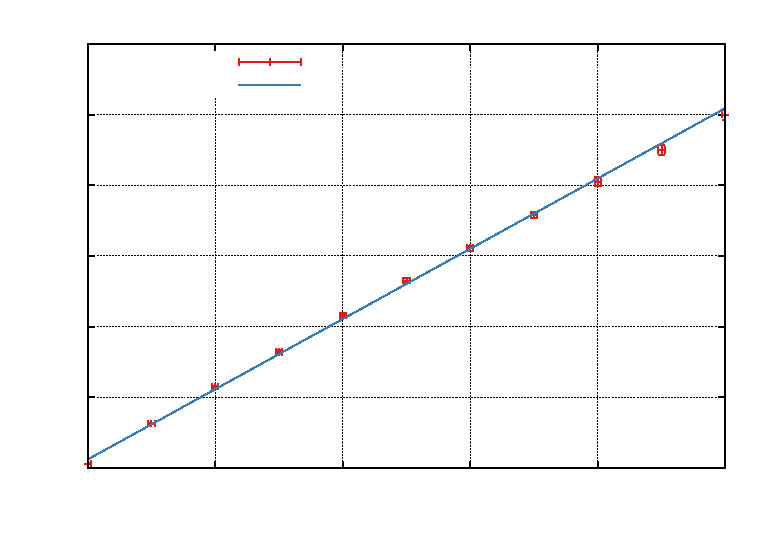
\includegraphics{./plots/abh_emissionsstrom/mo}}%
    \gplfronttext
  \end{picture}%
\endgroup

		\subcaption{Molybdän-Röhre}
		\label{fig:mo_emissionsstrom_dosis}
	\end{subfigure}
	
	\vspace{10mm}
	
	\begin{subfigure}[b]{\textwidth}
		\centering
		\begin{tabular}{SSSSSS}
	\toprule
	{$U / \si{kV}$} & {$\Delta U / \si{kV}$} & {$U_{I_\mathrm{C}} / \si{mV}$} & {$\Delta U_{I_\mathrm{C}} / \si{mV}$} & {$I_\mathrm{C} / \si{nA}$} & {$\Delta I_\mathrm{C} / \si{nA}$} \\ \midrule
	0.00   & 0.05      & 13        & 2            & 0.13      & 0.03         \\
	2.50   & 0.05      & 13        & 2            & 0.13      & 0.03         \\
	5.00   & 0.05      & 38        & 2            & 0.38      & 0.03         \\
	7.50   & 0.05      & 180       & 5            & 1.80      & 0.06         \\
	10.00  & 0.05      & 550       & 10           & 5.50      & 0.12         \\
	12.50  & 0.05      & 1090      & 10           & 10.90     & 0.15         \\
	15.00  & 0.05      & 1700      & 10           & 17.00     & 0.20         \\
	17.50  & 0.05      & 2330      & 10           & 23.30     & 0.26         \\
	20.00  & 0.05      & 2960      & 10           & 29.60     & 0.32         \\
	22.50  & 0.05      & 3510      & 10           & 35.10     & 0.37         \\
	25.00  & 0.05      & 3990      & 10           & 39.90     & 0.42         \\
	27.50  & 0.05      & 4390      & 10           & 43.90     & 0.46         \\
	30.00  & 0.05      & 4730      & 10           & 47.30     & 0.49         \\
	32.50  & 0.05      & 5020      & 10           & 50.20     & 0.52         \\
	35.00  & 0.05      & 5260      & 20           & 52.60     & 0.57         \\ \bottomrule
\end{tabular}
		\subcaption{Kupfer-Röhre}
		\label{fig:cu_emissionsstrom_dosis}
	\end{subfigure}
	\caption{Abhängigkeit der mittleren Ionendosisleistung $\braket{j}$ beziehungsweise der Äquivalentdosisleistung $\dot{H}$ vom Emissionsstrom $I_\mathrm{E}$ für verschiedene Röntgenröhren. Beide Messungen wurden bei maximaler Röhrenspannung $U=\SI{35}{kV}$ durchgeführt.}
	\label{fig:dosis_emissionsstrom}
\end{figure}
\begin{figure}[hp]
	\vspace{-10mm}
	
	\begin{subfigure}[b]{\textwidth}
		\centering
		% GNUPLOT: LaTeX picture with Postscript
\begingroup
  \makeatletter
  \providecommand\color[2][]{%
    \GenericError{(gnuplot) \space\space\space\@spaces}{%
      Package color not loaded in conjunction with
      terminal option `colourtext'%
    }{See the gnuplot documentation for explanation.%
    }{Either use 'blacktext' in gnuplot or load the package
      color.sty in LaTeX.}%
    \renewcommand\color[2][]{}%
  }%
  \providecommand\includegraphics[2][]{%
    \GenericError{(gnuplot) \space\space\space\@spaces}{%
      Package graphicx or graphics not loaded%
    }{See the gnuplot documentation for explanation.%
    }{The gnuplot epslatex terminal needs graphicx.sty or graphics.sty.}%
    \renewcommand\includegraphics[2][]{}%
  }%
  \providecommand\rotatebox[2]{#2}%
  \@ifundefined{ifGPcolor}{%
    \newif\ifGPcolor
    \GPcolortrue
  }{}%
  \@ifundefined{ifGPblacktext}{%
    \newif\ifGPblacktext
    \GPblacktexttrue
  }{}%
  % define a \g@addto@macro without @ in the name:
  \let\gplgaddtomacro\g@addto@macro
  % define empty templates for all commands taking text:
  \gdef\gplbacktext{}%
  \gdef\gplfronttext{}%
  \makeatother
  \ifGPblacktext
    % no textcolor at all
    \def\colorrgb#1{}%
    \def\colorgray#1{}%
  \else
    % gray or color?
    \ifGPcolor
      \def\colorrgb#1{\color[rgb]{#1}}%
      \def\colorgray#1{\color[gray]{#1}}%
      \expandafter\def\csname LTw\endcsname{\color{white}}%
      \expandafter\def\csname LTb\endcsname{\color{black}}%
      \expandafter\def\csname LTa\endcsname{\color{black}}%
      \expandafter\def\csname LT0\endcsname{\color[rgb]{1,0,0}}%
      \expandafter\def\csname LT1\endcsname{\color[rgb]{0,1,0}}%
      \expandafter\def\csname LT2\endcsname{\color[rgb]{0,0,1}}%
      \expandafter\def\csname LT3\endcsname{\color[rgb]{1,0,1}}%
      \expandafter\def\csname LT4\endcsname{\color[rgb]{0,1,1}}%
      \expandafter\def\csname LT5\endcsname{\color[rgb]{1,1,0}}%
      \expandafter\def\csname LT6\endcsname{\color[rgb]{0,0,0}}%
      \expandafter\def\csname LT7\endcsname{\color[rgb]{1,0.3,0}}%
      \expandafter\def\csname LT8\endcsname{\color[rgb]{0.5,0.5,0.5}}%
    \else
      % gray
      \def\colorrgb#1{\color{black}}%
      \def\colorgray#1{\color[gray]{#1}}%
      \expandafter\def\csname LTw\endcsname{\color{white}}%
      \expandafter\def\csname LTb\endcsname{\color{black}}%
      \expandafter\def\csname LTa\endcsname{\color{black}}%
      \expandafter\def\csname LT0\endcsname{\color{black}}%
      \expandafter\def\csname LT1\endcsname{\color{black}}%
      \expandafter\def\csname LT2\endcsname{\color{black}}%
      \expandafter\def\csname LT3\endcsname{\color{black}}%
      \expandafter\def\csname LT4\endcsname{\color{black}}%
      \expandafter\def\csname LT5\endcsname{\color{black}}%
      \expandafter\def\csname LT6\endcsname{\color{black}}%
      \expandafter\def\csname LT7\endcsname{\color{black}}%
      \expandafter\def\csname LT8\endcsname{\color{black}}%
    \fi
  \fi
    \setlength{\unitlength}{0.0500bp}%
    \ifx\gptboxheight\undefined%
      \newlength{\gptboxheight}%
      \newlength{\gptboxwidth}%
      \newsavebox{\gptboxtext}%
    \fi%
    \setlength{\fboxrule}{0.5pt}%
    \setlength{\fboxsep}{1pt}%
\begin{picture}(7200.00,5040.00)%
    \gplgaddtomacro\gplbacktext{%
      \csname LTb\endcsname%
      \put(550,704){\makebox(0,0)[r]{\strut{}$0$}}%
      \csname LTb\endcsname%
      \put(550,1383){\makebox(0,0)[r]{\strut{}$1$}}%
      \csname LTb\endcsname%
      \put(550,2061){\makebox(0,0)[r]{\strut{}$2$}}%
      \csname LTb\endcsname%
      \put(550,2740){\makebox(0,0)[r]{\strut{}$3$}}%
      \csname LTb\endcsname%
      \put(550,3418){\makebox(0,0)[r]{\strut{}$4$}}%
      \csname LTb\endcsname%
      \put(550,4097){\makebox(0,0)[r]{\strut{}$5$}}%
      \csname LTb\endcsname%
      \put(550,4775){\makebox(0,0)[r]{\strut{}$6$}}%
      \csname LTb\endcsname%
      \put(682,484){\makebox(0,0){\strut{}$0$}}%
      \csname LTb\endcsname%
      \put(1906,484){\makebox(0,0){\strut{}$0{,}2$}}%
      \csname LTb\endcsname%
      \put(3130,484){\makebox(0,0){\strut{}$0{,}4$}}%
      \csname LTb\endcsname%
      \put(4355,484){\makebox(0,0){\strut{}$0{,}6$}}%
      \csname LTb\endcsname%
      \put(5579,484){\makebox(0,0){\strut{}$0{,}8$}}%
      \csname LTb\endcsname%
      \put(6803,484){\makebox(0,0){\strut{}$1$}}%
    }%
    \gplgaddtomacro\gplfronttext{%
      \csname LTb\endcsname%
      \put(176,2739){\rotatebox{-270}{\makebox(0,0){\strut{}Ionisationsstrom $I_\mathrm{C} / \si{nA}$}}}%
      \put(3742,154){\makebox(0,0){\strut{}Emissionsstrom $I_\mathrm{E} / \si{mA}$}}%
      \csname LTb\endcsname%
      \put(2002,4602){\makebox(0,0)[r]{\strut{}Messdaten}}%
      \csname LTb\endcsname%
      \put(2002,4382){\makebox(0,0)[r]{\strut{}Anpassung}}%
    }%
    \gplbacktext
    \put(0,0){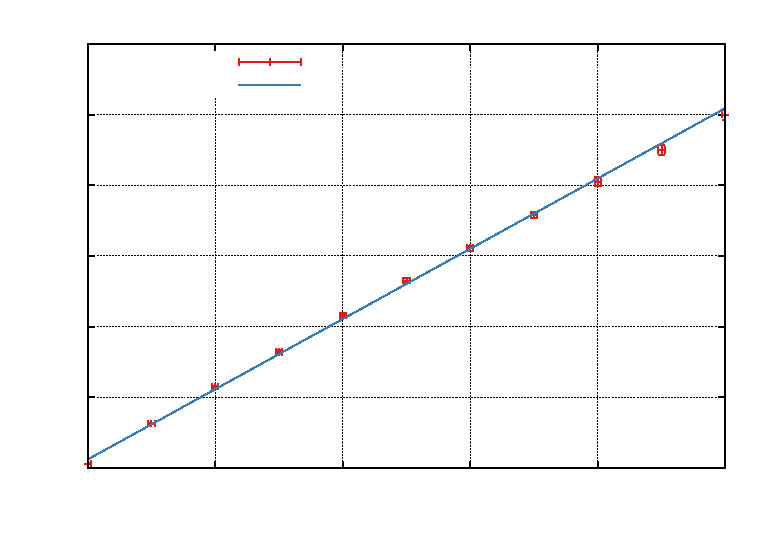
\includegraphics{./plots/abh_emissionsstrom/mo}}%
    \gplfronttext
  \end{picture}%
\endgroup

		\subcaption{Molybdän-Röhre mit charakteristischen Linien $\mathrm{K}_\alpha$ (\SI{17.4}{keV}) und $\mathrm{K}_\beta$ (\SI{19.6}{keV}) \cite{booklet}}
		\label{fig:mo_roehrenspannung_dosis}
	\end{subfigure}
	
	\vspace{2.5mm}
	
	\begin{subfigure}[b]{\textwidth}
		\centering
		\begin{tabular}{SSSSSS}
	\toprule
	{$U / \si{kV}$} & {$\Delta U / \si{kV}$} & {$U_{I_\mathrm{C}} / \si{mV}$} & {$\Delta U_{I_\mathrm{C}} / \si{mV}$} & {$I_\mathrm{C} / \si{nA}$} & {$\Delta I_\mathrm{C} / \si{nA}$} \\ \midrule
	0.00   & 0.05      & 13        & 2            & 0.13      & 0.03         \\
	2.50   & 0.05      & 13        & 2            & 0.13      & 0.03         \\
	5.00   & 0.05      & 38        & 2            & 0.38      & 0.03         \\
	7.50   & 0.05      & 180       & 5            & 1.80      & 0.06         \\
	10.00  & 0.05      & 550       & 10           & 5.50      & 0.12         \\
	12.50  & 0.05      & 1090      & 10           & 10.90     & 0.15         \\
	15.00  & 0.05      & 1700      & 10           & 17.00     & 0.20         \\
	17.50  & 0.05      & 2330      & 10           & 23.30     & 0.26         \\
	20.00  & 0.05      & 2960      & 10           & 29.60     & 0.32         \\
	22.50  & 0.05      & 3510      & 10           & 35.10     & 0.37         \\
	25.00  & 0.05      & 3990      & 10           & 39.90     & 0.42         \\
	27.50  & 0.05      & 4390      & 10           & 43.90     & 0.46         \\
	30.00  & 0.05      & 4730      & 10           & 47.30     & 0.49         \\
	32.50  & 0.05      & 5020      & 10           & 50.20     & 0.52         \\
	35.00  & 0.05      & 5260      & 20           & 52.60     & 0.57         \\ \bottomrule
\end{tabular}
		\subcaption{Kupfer-Röhre mit charakteristischen Linien $\mathrm{K}_\alpha$ (\SI{8.04}{keV}) und $\mathrm{K}_\beta$ (\SI{8.91}{keV}) \cite{booklet}}
		\label{fig:cu_roehrenspannung_dosis}
	\end{subfigure}
	\caption{Abhängigkeit der mittleren Ionendosisleistung $\braket{j}$ beziehungsweise der Äquivalentdosisleistung $\dot{H}$ von der Röhrenspannung $U$ für verschiedene Röntgenröhren. Beide Messungen wurden bei maximalem Emissionsstrom $I_\mathrm{E} = \SI{1.00}{mA}$ durchgeführt.}
	\label{fig:dosis_roehrenspannung}
\end{figure}

Die Form der Kurven wurde in den Abschnitten \ref{sec:abh_emissionsstrom} und \ref{sec:abh_roehrenspannung} bereits diskutiert, da sich der Kurvenverlauf lediglich in einer Skalierung der $y$-Achse unterscheidet\footnote{Die Fehler wurden nicht skaliert sondern durch \eqref{eq:fehler_dosisleistung} berechnet.} und soll hier nur kurz wiederholt werden.
Bei der Variation des Emissionsstroms der Röhre in Abbildung \ref{fig:dosis_emissionsstrom} ist ein linearer Verlauf zu erwarten, welcher beim Verlauf der Dosisleistung der Molybdän-Röhre zu beobachten ist.
Die Kupfer-Röhre hingegen weicht stark von dem erwarteten Verlauf ab, was auf die um einen Faktor 10 höhere Intensität der Röhre zurückzuführen sein könnte.
Der Grund dafür ist, dass im Kondensator soviel Ionisationen stattfinden, dass die stationäre Raumladung für einen Sättigung der Ionisationskammer sorgt.

Betrachtet man den Verlauf der Dosisleistungen bei Variation der Röhrenspannung $U$ in Abbildung \ref{fig:dosis_roehrenspannung}, so erkennt man einen starken Anstieg der Dosisleistung, sobald die Energie der durch die Röhrenspannung beschleunigten Elektronen groß genug ist, um charakteristische Röntgenlinien zu erzeugen.
Dazu wurden in der Abbildung die wichtigsten charakteristischen Linien der jeweiligen Anode markiert.

Abschließend soll das Volumen des Kondensators anhand der Dosisleistung in Überwachungs-, Kontroll- oder Sperrbereich klassifiziert werden.
In den Abbildungen kann man erkennen, dass die Ortsdosisleistung im Kondensator von der Größenordnung \SI{1}{\sievert\per\hour} ist, welche die Untergrenze für den Sperrbereich von \SI{3}{\milli\sievert\per\hour} stark überschreitet.
Demnach muss das Volumen des Kondensators als Sperrbereich klassifiziert werden.

\subsubsection{Bestimmung der Dosisleistung mit einem Stabdosimeter}
Zur Bestimmung der Dosisleistung mit dem Stabdosimeter (Messbereich: \num{0} bis \SI{10}{mSv}) wird der Kondensator im Experimentierraum des Röntgengeräts durch eine Experimentierschiene mit Längenskala ausgetauscht.
Der Nullpunkt der Skala liegt in \SI{110 +- 0.5}{mm} Entfernung von der Anode der Röntgenröhre.
Nun wird das Stabdosimeter etwa an der Position des Kondensators bei \SI{16 +- 0.1}{cm} auf der Skala der Schiene positioniert.
Damit ergibt sich ein Abstand von der Anode von:
\begin{align*}
	d = \SI{27.0 +- 0.2}{cm}
\end{align*}
Anschließend werden für die Molybdän- und die Kupfer-Röhre jeweils fünf Messungen der Dosis durchgeführt.
Dazu wird das Röntgengerät auf die Röhrenspannung $U = \SI{35}{kV}$, den Emissionsstrom $I_\mathrm{E} = \SI{1.00}{mA}$ und die Bestrahlungszeit $t = \SI{15}{s}$ gestellt.
Auf den Fehler der Bestrahlungszeit werden $\Delta t = \SI{1}{s}$ angenommen, da die Röntgenröhre nicht instantan ihre maximale Intensität erreicht.
In Tabelle \ref{tab:dosis_stabdosimeter} wurden die gemessenen Dosen aufgetragen.
\begin{table}[h]
	\centering
	\begin{tabular}{SS}
\toprule
{$D_\mathrm{Mo} / \si{mSv}$} & {$D_\mathrm{Cu} / \si{mSv}$} \\ \midrule
6.75    & 7.50    \\
7.00    & 7.25    \\
7.00    & 7.00    \\
6.75    & 7.25    \\
7.00    & 7.00    \\ \bottomrule
\end{tabular}
	\caption{Dosen im Strahlungsfeld der Röntgenröhre bei einer Bestrahlungszeit von $t=\SI{15}{s}$ mit Röhrenspannung $U=\SI{35}{kV}$ und Emissionsstrom $I_\mathrm{E} = \SI{1.00}{mA}$ bei einem Abstand $d=\SI{27 +- 0.2}{cm}$ von der Anode der Röntgenröhre.}
	\label{tab:dosis_stabdosimeter}
\end{table}
Bildung des Mittelwerts und der korrigierten Stichprobenvarianz der jeweiligen Messreihen liefern:
\begin{align*}
	D_\mathrm{Mo} = \SI{6.90 +- 0.14}{mSv} \\
	D_\mathrm{Cu} = \SI{7.20 +- 0.21}{mSv}
\end{align*}
Die Dosisleistung $\dot{D}$ kann nun durch Division durch die Bestrahlungszeit $t$ berechnet werden, wobei der Fehler durch Gauß'sche Fehlerfortpflanzung zu:
\begin{align}
	\Delta \dot{D} = \dot{D} \cdot \sqrt{\left( \frac{\Delta D}{D} \right)^2 + \left( \frac{\Delta t}{t} \right)^2}
\end{align}
gegeben ist.
Es folgen die Dosisleistungen:
\begin{align*}
	\dot{D}_\mathrm{Mo} = \SI{460 +- 10}{\micro\sievert\per\second} = \SI{1.656 +- 0.035}{\sievert\per\hour}\\
	\dot{D}_\mathrm{Cu} = \SI{480 +- 35}{\micro\sievert\per\second} = \SI{1.728 +- 0.126}{\sievert\per\hour}
\end{align*}
Leider kann weder die Größenordnung, noch der Faktor 10 höhere Intensität der Kupfer-Röhre reproduziert werden.

\subsubsection{Überprüfung des Abstandsquadratgesetzes}
Im Folgenden soll das Abstandsquadratgesetz der Kupfer-Röntgenröhre mithilfe eines Stabdosimeters überprüft werden.
Um eine Sättigung des Dosimeters im Experimentierraum zu vermeiden, musste der Emissionsstrom $I_\mathrm{E}$ der Röhre auf \SI{0.50}{mA} reduziert werden.
Weiterhin wird eine Röhrenspannung $U = \SI{35}{kV}$ und eine Bestrahlungszeit $t = \SI{15}{s}$ gewählt.
Die Messdaten wurden in Tabelle \ref{tab:abstandsquadrat} aufgetragen, wobei die Umrechnung von der Skala im Experimentierraum auf den Abstand des Dosimeters von der Röhrenanode $d$ bereits erfolgt ist.
\begin{table}[h]
	\centering
	\begin{tabular}{SSSS}
\toprule
{$d / \si{cm}$} & {$\Delta d / \si{cm}$} & {$D / \si{mSv}$} & {$\Delta D / \si{mSv}$} \\ \midrule
35 & 0.2       & 2.50    & 0.25       \\
33 & 0.2       & 2.75    & 0.25       \\
31 & 0.2       & 3.00    & 0.25       \\
29 & 0.2       & 3.25    & 0.25       \\
27 & 0.2       & 3.75    & 0.25       \\
25 & 0.2       & 4.50    & 0.25       \\
23 & 0.2       & 5.00    & 0.25       \\
21 & 0.2       & 5.50    & 0.25       \\
19 & 0.2       & 6.50    & 0.25       \\
17 & 0.2       & 7.25    & 0.25       \\
15 & 0.2       & 6.00    & 0.25       \\
13 & 0.2       & 4.25    & 0.25       \\ \bottomrule
\end{tabular}
	\caption{Messdaten der Dosis über eine Bestrahlungszeit von $t=\SI{15}{s}$ bei einem Emissionsstrom $I_\mathrm{E} = \SI{0.50}{mA}$ zur Bestätigung des Abstandsquadratsgesetzes. Der Abstand $d$ ist bereits in den Abstand Dosimeter-Anode umgerechnet worden.}
	\label{tab:abstandsquadrat}
\end{table}
\begin{figure}[h]
	\centering
	\begin{tabular}{SSSS}
\toprule
{$d / \si{cm}$} & {$\Delta d / \si{cm}$} & {$D / \si{mSv}$} & {$\Delta D / \si{mSv}$} \\ \midrule
35 & 0.2       & 2.50    & 0.25       \\
33 & 0.2       & 2.75    & 0.25       \\
31 & 0.2       & 3.00    & 0.25       \\
29 & 0.2       & 3.25    & 0.25       \\
27 & 0.2       & 3.75    & 0.25       \\
25 & 0.2       & 4.50    & 0.25       \\
23 & 0.2       & 5.00    & 0.25       \\
21 & 0.2       & 5.50    & 0.25       \\
19 & 0.2       & 6.50    & 0.25       \\
17 & 0.2       & 7.25    & 0.25       \\
15 & 0.2       & 6.00    & 0.25       \\
13 & 0.2       & 4.25    & 0.25       \\ \bottomrule
\end{tabular}
	\caption{Bestätigung des Abstandsquadratsgesetzes für die verwendete Kupfer-Röntgenröhre. Bei der Anpassung wurden die ersten beiden Messpunkte ignoriert.}
	\label{fig:abstandsquadrat}
\end{figure}
Die Messdaten wurden in Abbildung \ref{fig:abstandsquadrat} grafisch dargestellt, wobei die Anpassungshypothese:
\begin{align}
	D(d) = \frac{\lambda}{d^2} + D_0
\end{align}
gewählt wurde.
Die die Anpassung liefert die Parameter:
\begin{align*}
	\lambda &= \SI{1875 +- 95}{\milli\sievert\centi\metre\squared}\\
	D_0 &= \SI{1.15 +- 0.18}{\milli\sievert}
\end{align*}
Auffällig ist die starke Abweichung vom Abstandsquadratsgesetzes bei kleinen Abständen von der Anode.
Diese stammt daher, dass die Länge des Stabdosimeters nicht auf die Höhe der Rechteckblende im Röntgengerät abgestimmt wurde und daher die Ionisationskammer bei kleinen Abständen zumindest teilweise aus dem Strahlungsfeld hinausragt.
Dies ist ein rein geometrischer Effekt und sollte für größere Abstände vernachlässigbar sein, da das Strahlungsfeld dort eine höhere Aufweitung aufweist und somit die Ionisationskammer im Dosimeter komplett ausfüllt.

Unter Berücksichtigung dieses Effekts zeigt die Anpassung eine gute Übereinstimmung mit dem Abstandsquadratgesetzes.
Die Notwendigkeit eines konstanten Versatzes $D_0$ für einen guten Fit könnte ebenfalls auf geometrische Effekte zurückzuführen sein, wie z.B. die Abweichung von einer idealen Punktquelle oder den Weglängenunterschied (jeweils von der Quelle) zwischen der Mitte der Ionisationskammer und des oberen/unteren Randes zurückzuführen sein.

\subsection{Totzeit}

Da bei den weiteren Messungen das Geiger-Müller-Zählrohr verwendet wird, ist es notwendig, zunächst seine Totzeit abzuschätzen.
Dazu wird das Zählrohr auf dem Goniometer befestigt und zur Bestrahlung eine Röntgenröhre aus Kupfer mit davor sitzendem Kollimator (bei diesem Versuch wurde der Kollimator mit breitem Spalt verwendet) genutzt.
Das Zählrohr wird so positioniert, dass es sich gleich weit von der Goniometermitte entfernt befindet wie der Kollimator von der Goniometermitte (je ca. \num{5} bis \SI{7}{cm}).
Zur Messung wird die Zählrate über $\Delta t=\SI{30}{\second}$ gemittelt und eine Röhrenspannung von $U=\SI{35}{\kilo\volt}$ fest eingestellt, während der Emissionsstrom $I_\text{E}$ von \num{0} bis \SI{1}{\milli\ampere} variiert wird.
Das Maximum der Zählrate wird bei einer Winkeleinstellung des Zählrohrs von $\beta=\SI{-0.9}{\degree}$ lokalisiert und das Zählrohr für alle folgenden Messungen auf dieser Einstellung genutzt.
Die so gefundenen Zählraten in Abhängigkeit des Emissionsstroms sind in Tabelle \ref{tab:totzeit} festgehalten.
\begin{table}[ht]
	\centering
	% GNUPLOT: LaTeX picture with Postscript
\begingroup
  \makeatletter
  \providecommand\color[2][]{%
    \GenericError{(gnuplot) \space\space\space\@spaces}{%
      Package color not loaded in conjunction with
      terminal option `colourtext'%
    }{See the gnuplot documentation for explanation.%
    }{Either use 'blacktext' in gnuplot or load the package
      color.sty in LaTeX.}%
    \renewcommand\color[2][]{}%
  }%
  \providecommand\includegraphics[2][]{%
    \GenericError{(gnuplot) \space\space\space\@spaces}{%
      Package graphicx or graphics not loaded%
    }{See the gnuplot documentation for explanation.%
    }{The gnuplot epslatex terminal needs graphicx.sty or graphics.sty.}%
    \renewcommand\includegraphics[2][]{}%
  }%
  \providecommand\rotatebox[2]{#2}%
  \@ifundefined{ifGPcolor}{%
    \newif\ifGPcolor
    \GPcolortrue
  }{}%
  \@ifundefined{ifGPblacktext}{%
    \newif\ifGPblacktext
    \GPblacktexttrue
  }{}%
  % define a \g@addto@macro without @ in the name:
  \let\gplgaddtomacro\g@addto@macro
  % define empty templates for all commands taking text:
  \gdef\gplbacktext{}%
  \gdef\gplfronttext{}%
  \makeatother
  \ifGPblacktext
    % no textcolor at all
    \def\colorrgb#1{}%
    \def\colorgray#1{}%
  \else
    % gray or color?
    \ifGPcolor
      \def\colorrgb#1{\color[rgb]{#1}}%
      \def\colorgray#1{\color[gray]{#1}}%
      \expandafter\def\csname LTw\endcsname{\color{white}}%
      \expandafter\def\csname LTb\endcsname{\color{black}}%
      \expandafter\def\csname LTa\endcsname{\color{black}}%
      \expandafter\def\csname LT0\endcsname{\color[rgb]{1,0,0}}%
      \expandafter\def\csname LT1\endcsname{\color[rgb]{0,1,0}}%
      \expandafter\def\csname LT2\endcsname{\color[rgb]{0,0,1}}%
      \expandafter\def\csname LT3\endcsname{\color[rgb]{1,0,1}}%
      \expandafter\def\csname LT4\endcsname{\color[rgb]{0,1,1}}%
      \expandafter\def\csname LT5\endcsname{\color[rgb]{1,1,0}}%
      \expandafter\def\csname LT6\endcsname{\color[rgb]{0,0,0}}%
      \expandafter\def\csname LT7\endcsname{\color[rgb]{1,0.3,0}}%
      \expandafter\def\csname LT8\endcsname{\color[rgb]{0.5,0.5,0.5}}%
    \else
      % gray
      \def\colorrgb#1{\color{black}}%
      \def\colorgray#1{\color[gray]{#1}}%
      \expandafter\def\csname LTw\endcsname{\color{white}}%
      \expandafter\def\csname LTb\endcsname{\color{black}}%
      \expandafter\def\csname LTa\endcsname{\color{black}}%
      \expandafter\def\csname LT0\endcsname{\color{black}}%
      \expandafter\def\csname LT1\endcsname{\color{black}}%
      \expandafter\def\csname LT2\endcsname{\color{black}}%
      \expandafter\def\csname LT3\endcsname{\color{black}}%
      \expandafter\def\csname LT4\endcsname{\color{black}}%
      \expandafter\def\csname LT5\endcsname{\color{black}}%
      \expandafter\def\csname LT6\endcsname{\color{black}}%
      \expandafter\def\csname LT7\endcsname{\color{black}}%
      \expandafter\def\csname LT8\endcsname{\color{black}}%
    \fi
  \fi
    \setlength{\unitlength}{0.0500bp}%
    \ifx\gptboxheight\undefined%
      \newlength{\gptboxheight}%
      \newlength{\gptboxwidth}%
      \newsavebox{\gptboxtext}%
    \fi%
    \setlength{\fboxrule}{0.5pt}%
    \setlength{\fboxsep}{1pt}%
\begin{picture}(7200.00,5040.00)%
    \gplgaddtomacro\gplbacktext{%
      \csname LTb\endcsname%
      \put(1210,704){\makebox(0,0)[r]{\strut{}$0$}}%
      \csname LTb\endcsname%
      \put(1210,1213){\makebox(0,0)[r]{\strut{}$100000$}}%
      \csname LTb\endcsname%
      \put(1210,1722){\makebox(0,0)[r]{\strut{}$200000$}}%
      \csname LTb\endcsname%
      \put(1210,2231){\makebox(0,0)[r]{\strut{}$300000$}}%
      \csname LTb\endcsname%
      \put(1210,2740){\makebox(0,0)[r]{\strut{}$400000$}}%
      \csname LTb\endcsname%
      \put(1210,3248){\makebox(0,0)[r]{\strut{}$500000$}}%
      \csname LTb\endcsname%
      \put(1210,3757){\makebox(0,0)[r]{\strut{}$600000$}}%
      \csname LTb\endcsname%
      \put(1210,4266){\makebox(0,0)[r]{\strut{}$700000$}}%
      \csname LTb\endcsname%
      \put(1210,4775){\makebox(0,0)[r]{\strut{}$800000$}}%
      \csname LTb\endcsname%
      \put(1342,484){\makebox(0,0){\strut{}0{,}0}}%
      \csname LTb\endcsname%
      \put(2335,484){\makebox(0,0){\strut{}0{,}2}}%
      \csname LTb\endcsname%
      \put(3328,484){\makebox(0,0){\strut{}0{,}4}}%
      \csname LTb\endcsname%
      \put(4321,484){\makebox(0,0){\strut{}0{,}6}}%
      \csname LTb\endcsname%
      \put(5314,484){\makebox(0,0){\strut{}0{,}8}}%
      \csname LTb\endcsname%
      \put(6307,484){\makebox(0,0){\strut{}1{,}0}}%
    }%
    \gplgaddtomacro\gplfronttext{%
      \csname LTb\endcsname%
      \put(176,2739){\rotatebox{-270}{\makebox(0,0){\strut{}Zählrate $R$ / \si{\per\second}}}}%
      \put(4072,154){\makebox(0,0){\strut{}Emissionsstrom $I_\text{E}$ / \si{mA}}}%
      \csname LTb\endcsname%
      \put(2662,4602){\makebox(0,0)[r]{\strut{}Messwerte}}%
      \csname LTb\endcsname%
      \put(2662,4382){\makebox(0,0)[r]{\strut{}Anpassung}}%
    }%
    \gplbacktext
    \put(0,0){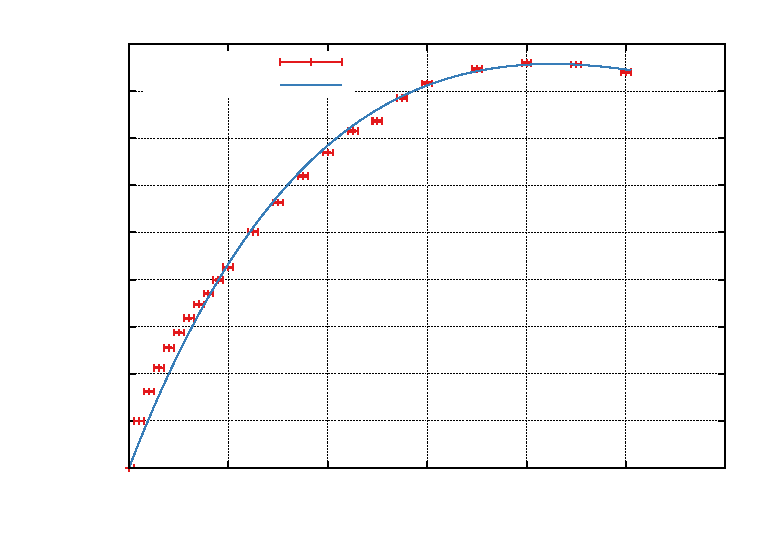
\includegraphics{./plots/totzeit}}%
    \gplfronttext
  \end{picture}%
\endgroup

	\caption{Messwerte zur Abschätzung der Totzeit, gezeigt ist die Abhängigkeit der Zählrate vom Emissionsstrom.}
	\label{tab:totzeit}
\end{table}
Der Fehler von $I_\text{E}$ wurde dabei wie oben auf \SI{0.005}{\milli\ampere} geschätzt, für den Fehler von $R$ wurde Gauß'sche Fehlerfortpflanzung genutzt.
Dabei gilt:
\begin{align}
	R = \frac{N}{T}\qquad\text{$N$: Anzahl Ereignisse, $T$: gemessene Zeit}
\end{align}
Mit Gauß'scher Fehlerfortpflanzung folgt unter der Annahme, dass der Fehler der Zeit $\Delta T=0$ ist:
\begin{align}
	\Delta R &= \sqrt{\frac{(\Delta N)^2}{T^2}} &\qquad \Delta N =\sqrt{N} \\
				 &= \sqrt{\frac{N}{T^2}} &\qquad \frac{N}{T}= R\\
				 &= \sqrt{\frac{R}{T}} \label{eq:zählrate_fehler}
\end{align}
Grafisch aufgetragen erhält man aus diesen die Abbildung \ref{fig:totzeit}.
\begin{figure}[ht]
	\centering
	% GNUPLOT: LaTeX picture with Postscript
\begingroup
  \makeatletter
  \providecommand\color[2][]{%
    \GenericError{(gnuplot) \space\space\space\@spaces}{%
      Package color not loaded in conjunction with
      terminal option `colourtext'%
    }{See the gnuplot documentation for explanation.%
    }{Either use 'blacktext' in gnuplot or load the package
      color.sty in LaTeX.}%
    \renewcommand\color[2][]{}%
  }%
  \providecommand\includegraphics[2][]{%
    \GenericError{(gnuplot) \space\space\space\@spaces}{%
      Package graphicx or graphics not loaded%
    }{See the gnuplot documentation for explanation.%
    }{The gnuplot epslatex terminal needs graphicx.sty or graphics.sty.}%
    \renewcommand\includegraphics[2][]{}%
  }%
  \providecommand\rotatebox[2]{#2}%
  \@ifundefined{ifGPcolor}{%
    \newif\ifGPcolor
    \GPcolortrue
  }{}%
  \@ifundefined{ifGPblacktext}{%
    \newif\ifGPblacktext
    \GPblacktexttrue
  }{}%
  % define a \g@addto@macro without @ in the name:
  \let\gplgaddtomacro\g@addto@macro
  % define empty templates for all commands taking text:
  \gdef\gplbacktext{}%
  \gdef\gplfronttext{}%
  \makeatother
  \ifGPblacktext
    % no textcolor at all
    \def\colorrgb#1{}%
    \def\colorgray#1{}%
  \else
    % gray or color?
    \ifGPcolor
      \def\colorrgb#1{\color[rgb]{#1}}%
      \def\colorgray#1{\color[gray]{#1}}%
      \expandafter\def\csname LTw\endcsname{\color{white}}%
      \expandafter\def\csname LTb\endcsname{\color{black}}%
      \expandafter\def\csname LTa\endcsname{\color{black}}%
      \expandafter\def\csname LT0\endcsname{\color[rgb]{1,0,0}}%
      \expandafter\def\csname LT1\endcsname{\color[rgb]{0,1,0}}%
      \expandafter\def\csname LT2\endcsname{\color[rgb]{0,0,1}}%
      \expandafter\def\csname LT3\endcsname{\color[rgb]{1,0,1}}%
      \expandafter\def\csname LT4\endcsname{\color[rgb]{0,1,1}}%
      \expandafter\def\csname LT5\endcsname{\color[rgb]{1,1,0}}%
      \expandafter\def\csname LT6\endcsname{\color[rgb]{0,0,0}}%
      \expandafter\def\csname LT7\endcsname{\color[rgb]{1,0.3,0}}%
      \expandafter\def\csname LT8\endcsname{\color[rgb]{0.5,0.5,0.5}}%
    \else
      % gray
      \def\colorrgb#1{\color{black}}%
      \def\colorgray#1{\color[gray]{#1}}%
      \expandafter\def\csname LTw\endcsname{\color{white}}%
      \expandafter\def\csname LTb\endcsname{\color{black}}%
      \expandafter\def\csname LTa\endcsname{\color{black}}%
      \expandafter\def\csname LT0\endcsname{\color{black}}%
      \expandafter\def\csname LT1\endcsname{\color{black}}%
      \expandafter\def\csname LT2\endcsname{\color{black}}%
      \expandafter\def\csname LT3\endcsname{\color{black}}%
      \expandafter\def\csname LT4\endcsname{\color{black}}%
      \expandafter\def\csname LT5\endcsname{\color{black}}%
      \expandafter\def\csname LT6\endcsname{\color{black}}%
      \expandafter\def\csname LT7\endcsname{\color{black}}%
      \expandafter\def\csname LT8\endcsname{\color{black}}%
    \fi
  \fi
    \setlength{\unitlength}{0.0500bp}%
    \ifx\gptboxheight\undefined%
      \newlength{\gptboxheight}%
      \newlength{\gptboxwidth}%
      \newsavebox{\gptboxtext}%
    \fi%
    \setlength{\fboxrule}{0.5pt}%
    \setlength{\fboxsep}{1pt}%
\begin{picture}(7200.00,5040.00)%
    \gplgaddtomacro\gplbacktext{%
      \csname LTb\endcsname%
      \put(1210,704){\makebox(0,0)[r]{\strut{}$0$}}%
      \csname LTb\endcsname%
      \put(1210,1213){\makebox(0,0)[r]{\strut{}$100000$}}%
      \csname LTb\endcsname%
      \put(1210,1722){\makebox(0,0)[r]{\strut{}$200000$}}%
      \csname LTb\endcsname%
      \put(1210,2231){\makebox(0,0)[r]{\strut{}$300000$}}%
      \csname LTb\endcsname%
      \put(1210,2740){\makebox(0,0)[r]{\strut{}$400000$}}%
      \csname LTb\endcsname%
      \put(1210,3248){\makebox(0,0)[r]{\strut{}$500000$}}%
      \csname LTb\endcsname%
      \put(1210,3757){\makebox(0,0)[r]{\strut{}$600000$}}%
      \csname LTb\endcsname%
      \put(1210,4266){\makebox(0,0)[r]{\strut{}$700000$}}%
      \csname LTb\endcsname%
      \put(1210,4775){\makebox(0,0)[r]{\strut{}$800000$}}%
      \csname LTb\endcsname%
      \put(1342,484){\makebox(0,0){\strut{}0{,}0}}%
      \csname LTb\endcsname%
      \put(2335,484){\makebox(0,0){\strut{}0{,}2}}%
      \csname LTb\endcsname%
      \put(3328,484){\makebox(0,0){\strut{}0{,}4}}%
      \csname LTb\endcsname%
      \put(4321,484){\makebox(0,0){\strut{}0{,}6}}%
      \csname LTb\endcsname%
      \put(5314,484){\makebox(0,0){\strut{}0{,}8}}%
      \csname LTb\endcsname%
      \put(6307,484){\makebox(0,0){\strut{}1{,}0}}%
    }%
    \gplgaddtomacro\gplfronttext{%
      \csname LTb\endcsname%
      \put(176,2739){\rotatebox{-270}{\makebox(0,0){\strut{}Zählrate $R$ / \si{\per\second}}}}%
      \put(4072,154){\makebox(0,0){\strut{}Emissionsstrom $I_\text{E}$ / \si{mA}}}%
      \csname LTb\endcsname%
      \put(2662,4602){\makebox(0,0)[r]{\strut{}Messwerte}}%
      \csname LTb\endcsname%
      \put(2662,4382){\makebox(0,0)[r]{\strut{}Anpassung}}%
    }%
    \gplbacktext
    \put(0,0){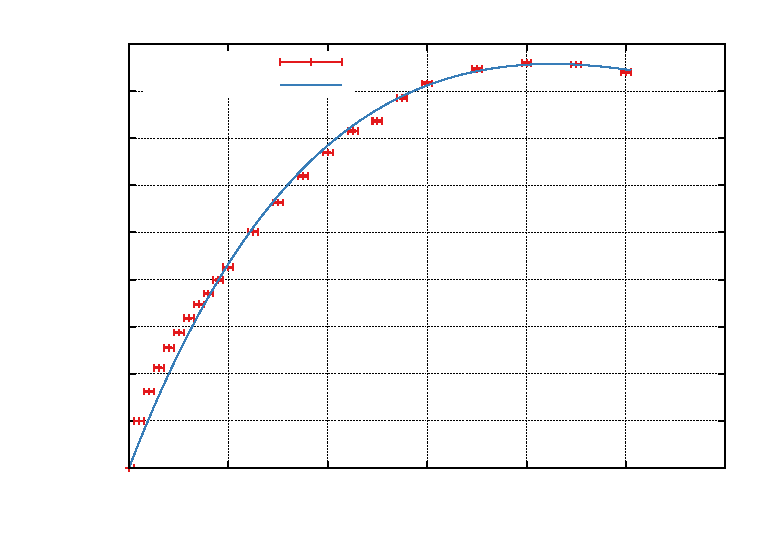
\includegraphics{./plots/totzeit}}%
    \gplfronttext
  \end{picture}%
\endgroup

	\caption{Abhängigkeit der Zählrate vom Emissionsstrom zur Abschätzung der Totzeit. Es handelt sich um ein paralysierendes System.}
	\label{fig:totzeit}
\end{figure}
Es ist deutlich zu sehen, dass es sich bei dem beobachteten Aufbau um ein paralysierendes System handelt.
Dies ist erkennbar an der Tatsache, dass die Zählrate nicht wie für ein nicht-paralysierendes System erwartet in Sättigung geht, sondern nach Erreichen eines Maximums bei zunehmendem Emissionsstrom wieder abnimmt.
Eine Anpassung der Form wie \eqref{eq:totzeit_paralysierend}, die bereits in Abbildung \ref{fig:totzeit} durchgeführt wurde stärkt diese Annahme.
Dabei wird davon ausgegangen, dass die echte Zählrate $m$ proportional zum Emissionsstrom ist (Proportionalitätskonstante $\lambda$ aus der Anpassung: $\lambda$=\SI{27169.8+-339.3}{\per\second\per\milli\ampere}).
Aus der Anpassung kann ebenfalls mit \eqref{eq:totzeit_paralysierend} die Totzeit $\tau$ des paralysierenden Systems recht gut bestimmt werden zu:
\begin{align}
\tau = \SI{4.29 +- 0.02e-5}{\second}
\end{align}

\subsection{Abschirmung}

Die Messungen zu diesem Abschnitt wurden mit den gleichen Einstellungen wie oben durchgeführt ($\Delta t=\SI{30}{\second}, U=\SI{35}{\kilo\volt}$, maximale Zählrate bei $\beta=\SI{-0.9}{\degree}$).
Nun wird jedoch vor dem Zählrohr einer der beiden Absorbersätze auf dem Targethalter eingebaut und die Zählrate dahinter gemessen.
Dafür wird der Emissionsstrom so gewählt, dass keine Totzeitkorrektur durchgeführt werden muss, hier wurde für alle Messungen eine maximale Zählrate von ca. \SI{400}{\per\second} angestrebt.
Der Targethalter wurde dann in Schritten von $\Delta\alpha=$\SI{10}{\degree} gedreht, um für das jeweilige Material bzw. die jeweilige Dicke der Aluminiumschicht die Zählrate zu bestimmen.
Die Messungen wurden einmal mit und einmal ohne Zirkonfilter duchgeführt.
Dieser filtert den kurzwelligen Anteil des Spektrums der erzeugten Bremsstrahlung aus.
Die so gefundenen Messwerte sind in Tabelle \ref{tab:absorber} und \ref{tab:absorber_zr} zu finden.
Dabei wurde der Fehler des Emissionsstroms erneut auf \SI{0.01}{\milli\ampere} abgeschätzt und der Fehler der Zählrate mit \eqref{eq:zählrate_fehler} berechnet.

\subsubsection{Korrigierte Zählraten}

\subsubsection{Transmissionen für Absorber}

\subsubsection{Transmissionskoeffizienten}

\subsection{Computertomographie}

Zum Abschluss wurde mit einem Computertomographie-Gerät ein CT-Scan eines gefriergetrockneten Frosches aufgenommen.
Dazu wird das zu untersuchende Objekt in einer für Röntgenstrahlung beinahe durchsichtigen Styroporkugel so gelagert, dass es sich nicht bewegen kann (hierzu wurde genügend Watte in den Hohlraum der Styroporkugel gegeben).
Anschließend kann das Objekt an dem Goniometer montiert werden.
Neben dem Röntgengerät wird das CT-Modul mit der Kamera aufgebaut, so dass die beiden Geräte möglichst dicht aneinander stehen, um kein Licht von außen in das CT-Modul gelangen zu lassen (das Röntgengerät ist mit einer Fluoreszenzschicht am Übergang ausgestattet, auf dem das mit der Kamera aufzunehmende Bild entsteht).
Nach dem Start des Computertomographie-Programms werden dort die Parameter des Aufbaus (insbesondere der Abstand des Targets von der Kamera) sowie die gewünschten Einstellungen der Röntgenröhre eingegeben.
Für den hier durchgeführten CT-Scan wurde eine Röhrenspannung von \SI{35}{\kilo\volt} bei \SI{1}{\milli\ampere} Emissionsstrom an der Molybdän-Röntgenröhre angelegt.
Nach Bildjustage und Kalibrierung der Kamera zur optimalen Aufnahme des Fluoreszenzschirms (Verzeichnungskorrektur, Größe des Schirms etc.) werden die Aufnahmeparameter, namentlich die Anzahl der Projektionen, ihre Größe und die Rekonstruktionsgröße gewählt.
Die Projektionsgröße wurde dabei auf \SI{250x250}{px} eingestellt, da so das ganze Objekt in dem aufgenommenen Bildbereich liegt, größere Projektionen hätten zusätzlich nur störende Aufnahmen der Befestigungen aufgenommen und keine Verbesserung des Bildes bewirkt.
Den Hinweisen des Programms folgend wurde die Rekonstruktionsgröße kleiner als die Projektionsgröße gewählt, auf \SI{240x240x240}{px}.

Zur Drehachsenkorrektur wurde die Anzahl Projektionen zunächst gering gewählt (verschiedene Messungen mit maximal \num{45} Projektionen) und die Aufnahme gestartet.
Ausgehend von dem aufgenommenen Bild kann durch das Programm eine Korrektur der Drehachse berechnet und die Kamera entsprechend manuell justiert werden, so dass keine Doppelkonturen mehr im Bild zu erkennen sind.
Nach mehreren Aufnahmen und anschließender Korrektur konnte so eine gute Justierung erreicht werden.

\subsubsection{Aufnahme und Rekonstruktion}
\label{ct_aufnahme}

Im Folgenden soll das allgemeine Vorgehen bei einer Computertomographieaufnahme anhand des im Versuch durchgeführten Scans beschrieben werden.
Nach entsprechender Justierung (s.o.) wird für eine qualitativ gute Aufnahme die Anzahl der Projektionen möglichst hoch gewählt.
Sie gibt die Menge der Bilder an, die während einer kompletten Umdrehung des Objekts aufgenommen werden.
In dem Versuch wurden \num{720} Projektionen eingestellt, was einer Winkelschrittweite pro Bild von $\Delta\alpha=$\SI{0.5}{\degree} entspricht.
Ein paar ausgewählte Einzelprojektionen sind in Abbildung \ref{fig:ct_projektionen} dargestellt.
\begin{figure}[ht]
	\begin{subfigure}[c]{0.5\textwidth}
		\centering
		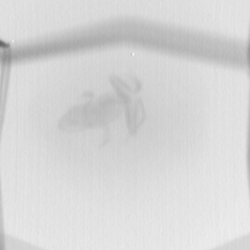
\includegraphics[width=0.9\textwidth]{./figures/ct/Projection2_5.png}
		\subcaption{Projektion für $\alpha$=\SI{2.5}{\degree}}
	\end{subfigure}
	\begin{subfigure}[c]{0.5\textwidth}
		\centering
		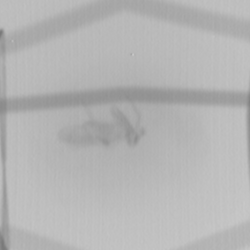
\includegraphics[width=0.9\textwidth]{./figures/ct/Projection264.png}
		\subcaption{Projektion für $\alpha$=\SI{264}{\degree}}
	\end{subfigure}
	\caption{Beispielhafte Projektionen für unterschiedliche Drehwinkel $\alpha$ des Objekts.}
	\label{fig:ct_projektionen}
\end{figure}
Diese Projektionen entsprechen jeweils einer gewöhnlichen Röntgenaufnahme eines Objekts mit dafür typischen Kontrasten.
Zur Kontrastverbesserung werden die einzelnen Projektionen bei der Computertomographie überlagert und so ein dreidimensionales kontrastreiches Bild erstellt.
Bei der hier genutzten Software und Vorgehensweise wird das Objekt mittels s.g. Rückprojektion (engl. \emph{back projection}) aus den einzelnen Aufnahmen rekonstruiert.
Die allgemeine Vorgehensweise\footnote{Dabei wird vereinfachend davon ausgegangen, dass das Bild in einem geeigneten Detektor entsteht, wobei dieser in dem Versuch aus Fluoreszenzschirm und Kamera zusammengesetzt ist.} umfasst dabei folgende Punkte (nach \cite{kalender}, Abb. 1.7):
\begin{enumerate}
	\item \textbf{Aufnahme der Projektionen} Hierbei entstehen gerasterte Bilder (d.h. diskrete Pixel), wobei jedem Pixel eine Helligkeit, abhängig von der Transmission des Strahls in diesem Bildpunkt, zugeordnet wird.
	\item \textbf{Filterung mit geeignetem Faltungskern} Die Projektionen werden mit einem Kern gefaltet, der je nach Anwendung gewählt werden kann.
	Er erzeugt Über- und Unterschwinger an Kanten, um diese beispielsweise zu betonen oder zu glätten (siehe auch Abb. \ref{fig:ct_faltung}).
	\begin{figure}[ht]
		\centering
		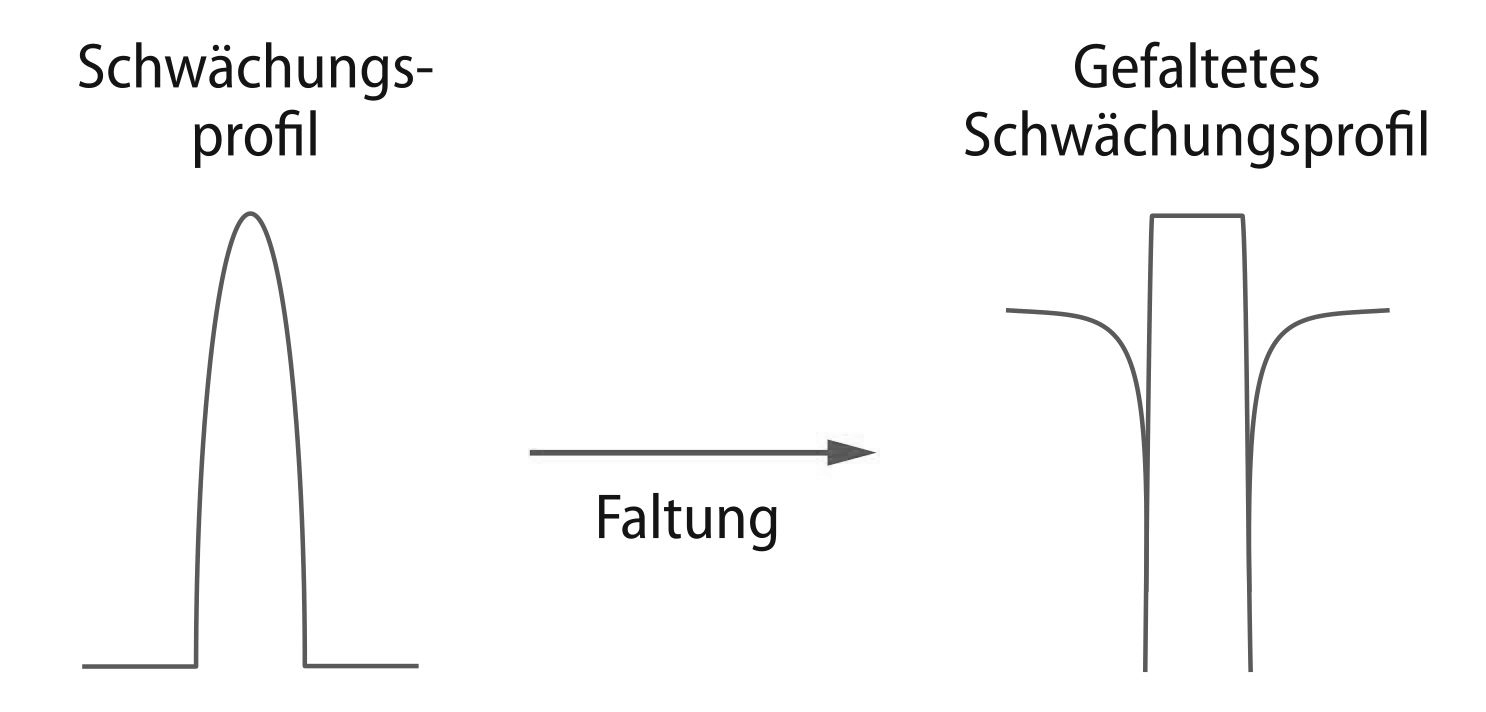
\includegraphics[width=0.7\textwidth]{./figures/ct/faltung.jpg}
		\caption{Hochpassfilterung durch Faltung des Schwächungsprofils mit einem geeigneten Faltungskern (aus \cite{alkadhi}).}
		\label{fig:ct_faltung}
	\end{figure}
	Aus Implementierungsgründen wird das Bild vorher fouriertransformiert, da die Faltung dadurch in eine deutlich schneller zu berechnende Multiplikation übergeht und anschließend rücktransformiert.
	\item \textbf{Überlagerung der Projektionen} Zur dreidimensionalen Rekonstruktion werden die einzelnen Projektionen entsprechend ihres zugehörigen Aufnahmewinkels überlagert.
	Siehe dazu auch die schematische Abbildung \ref{fig:ct_überlagerung}.
	\begin{figure}[ht]
		\centering
		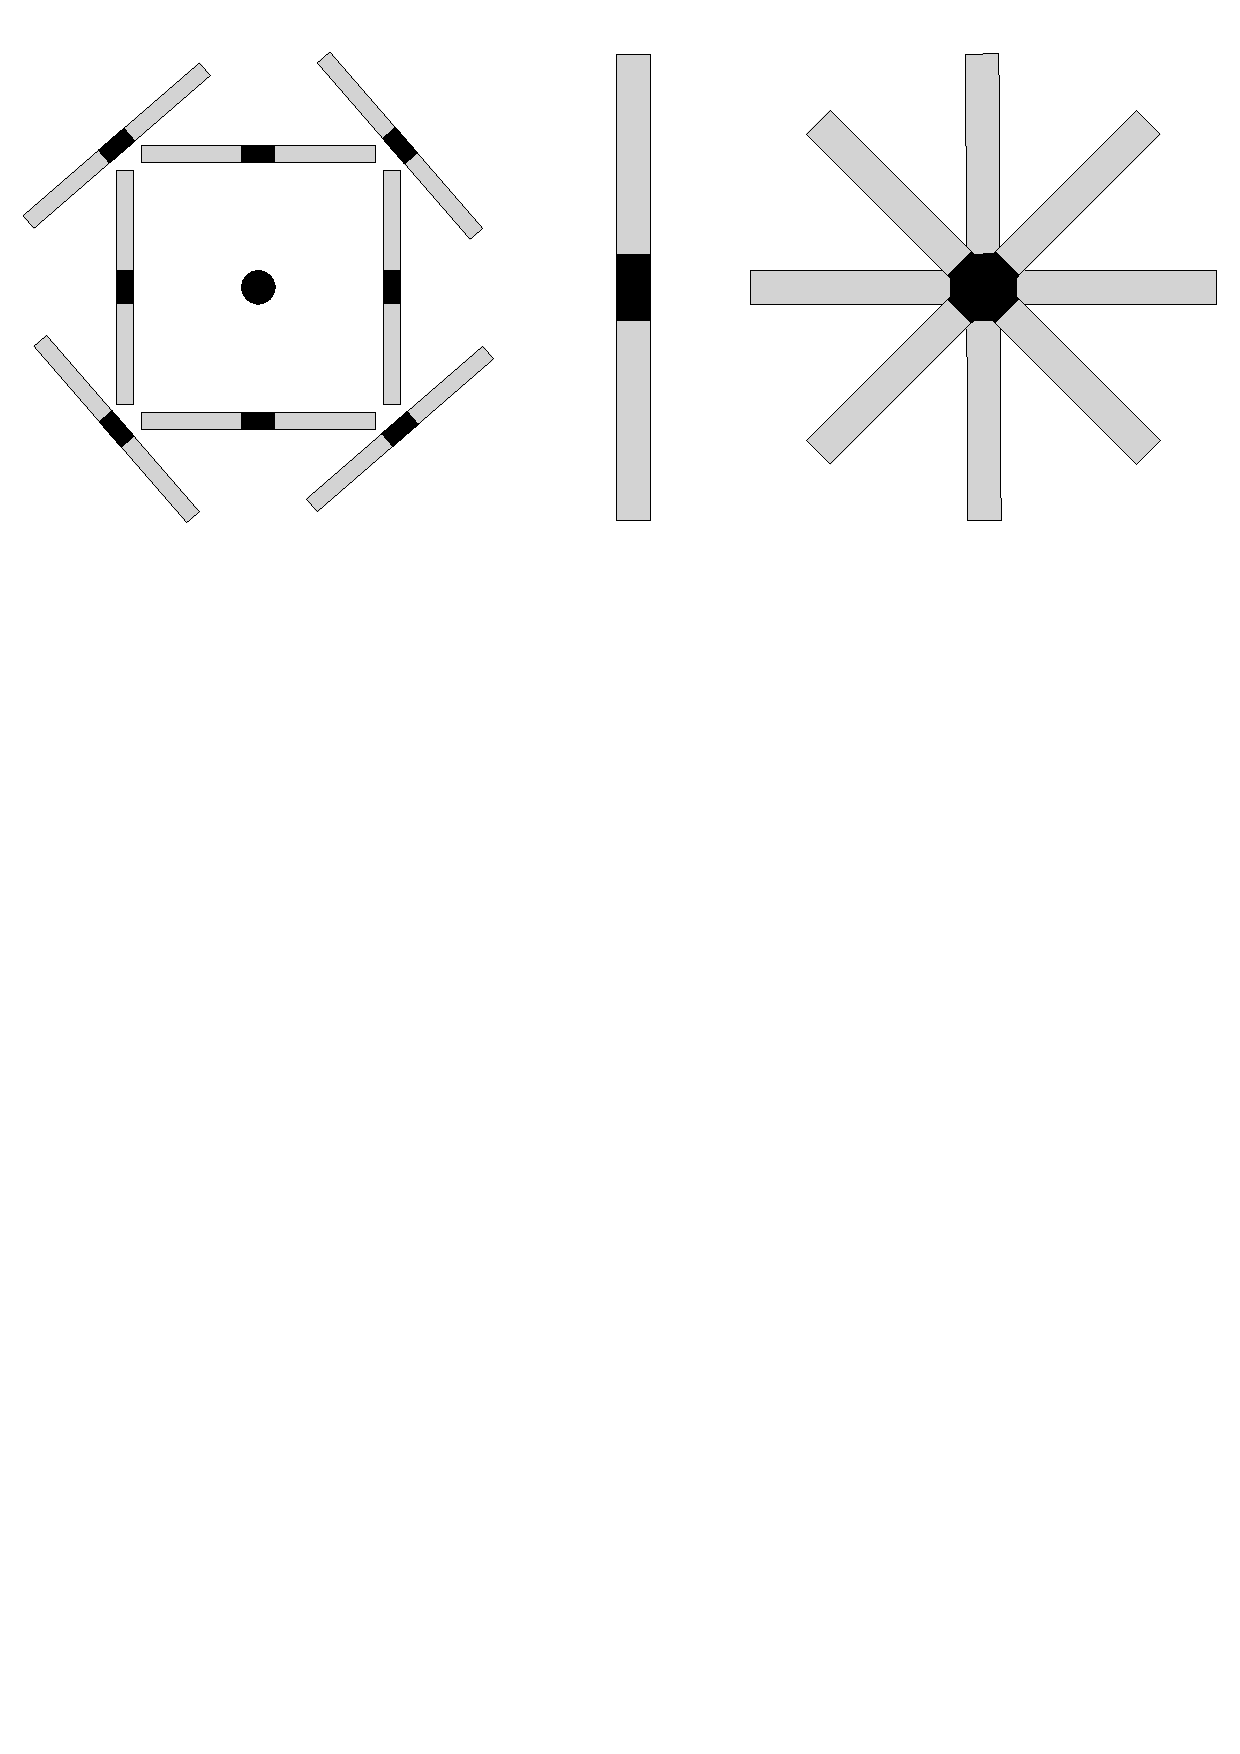
\includegraphics[width=0.8\textwidth]{./figures/ct/ueberlagerung.pdf}
		\caption{Schematische Darstellung zur Überlagerung einzelner Projektionen in Draufsicht. Links: Aufnahme von 8 Projektionen eines Zylinders. Mitte: Einzelne Projektion, vgl. auch Abb. \ref{fig:ct_faltung}. Rechts: Überlagerung der Projektionen. Es ist offensichtlich, dass mit steigender Anzahl Projektionen die Rekonstruktion immer besser wird.}
		\label{fig:ct_überlagerung}
	\end{figure}
\end{enumerate}
Da die Projektionen während der Rekonstruktion modifiziert werden, indem sie durch eine Faltung eine Filterung erfahren wird das Verfahren auch als gefilterte Rückprojektion bezeichnet.

Mathematisch wird die Projektion durch eine s.g. Radontransformation beschrieben, die die Objektfunktion $f(x, y)$ in eine Projektionsfunktion $p(\vartheta, \xi)$ überführt.
Die Variablen $\vartheta$ und $\xi$ parametrisieren den Röntgenstrahl in Polarkoordinaten, wobei der Ursprung im Zentrum des Objekts liegt.
Dann gilt:
\begin{align}
\xi=x\,\cos\vartheta + y\,\sin\vartheta
\end{align}
Die Projektionsfunktion ergibt sich dann mit der Radontransformation:
\begin{align}
p(\vartheta, \xi)=\int\mathrm{d}x\mathrm{d}y\,f(x, y)\,\delta(x\,\cos\vartheta + y\,\sin\vartheta - \xi)
\end{align}
Hierbei bezeichnet $\delta$ die Dirac'sche Deltafunktion.
Zur Rekonstruktion ist es nötig, die inverse Radontransformation zu bestimmen, um von $p(\vartheta, \xi)$ auf die Objektfunktion zu schließen.
Analytisch erhält man bei der Herleitung der inversen Radontransformation das Fourier-Slice-Theorem:
\begin{align}
F(u\,\cos\vartheta, u\,\sin\vartheta)=P(\vartheta, u)
\end{align}
Mit Großbuchstaben bezeichnete Funktionen sind dabei Fouriertransformierte, so dass man erhält, dass die zweidimensionale Fouriertransformation der Objektfunktion in Polarkoordinaten $f(u\,\cos\vartheta, u\,\sin\vartheta)$ gleich der Fouriertransformation der Projektionsfunktion bezüglich $\xi$ ist.
Ausgehend von diesem Theorem kann man über inverse Fouriertransformationen und den Faltungssatz zeigen, dass die inverse Radontransformation gegeben ist durch\cite{kalender}:
\begin{align}
f(x,y)=\int_{0}^{\pi}\left.\mathrm{d}\vartheta\,P(\vartheta, \xi)*k(\xi)\right|_{\xi=x\,\cos\vartheta + y\,\sin\vartheta}
\end{align}
$k(\xi)$ beschreibt hier den Faltungskern für die Filterung.

\subsubsection{Rekonstruiertes Objekt}
Das durch die Software rekonstruierte Objekt ist in Abbildung \ref{fig:ct_frosch} dargestellt.
\begin{figure}[ht]
	\centering
	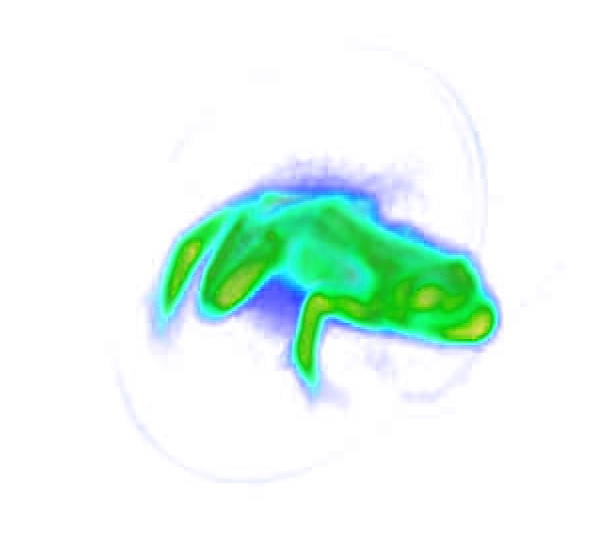
\includegraphics[width=0.7\textwidth]{./figures/ct/frosch.jpg}
	\caption{Rekonstruiertes Modell des Froschs}
	\label{fig:ct_frosch}
\end{figure}
Der Frosch ist dabei sehr deutlich zu erkennen, die gewählte Anzahl Projektionen sorgt offensichtlich für eine qualitativ gute Rekonstruktion.
Die nah am Frosch befindliche Watte zur stabilen Lagerung ist ebenfalls gut erkennbar, sowie ein außen liegender Ring der Befestigung.

\subsubsection{Strahlenbelastung bei CT-Aufnahmen}
Die folgenden Überlegungen sollen eine Einschätzung der Strahlenbelastung bei einem CT-Scan liefern, in der Praxis jedoch sind konkrete aufgenommene Dosen nur schwer zu berechnen und von vielen verschiedenen Faktoren abhängig.
Aufgrund der begrenzten Verfügbarkeit allgemeiner Quellen sind die angegebenen Informationen in den meisten Fällen auf Computertomographiegeräte für medizinische Anwendungen bezogen.
Im Gegesatz zu gewöhnlichen Röntgenaufnahmen, bei denen die Dosis etwa exponentiell mit der Dicke des durchstrahlten Objektes abnimmt (die Dosis ist proportional zur Intensität) ergibt sich für ein in der Computertomographie aufgenommenes Objekt oder auch Patienten bei medizinischen Anwendungen eine andere Dosisverteilung.
Durch eine Messung über \SI{360}{\degree} addieren sich die pro Einzelbild aufgenommenen Dosen, so dass sich insgesamt eine homogene Verteilung ergibt.
Bei schichtweisen CT-Aufnahmen eines Objekts, bei dem das in \ref{ct_aufnahme} beschriebene Vorgehen für jede Schicht durchgeführt wird (die Schichten, engl. \emph{slices} sind in $z$-Richtung aneinandergereiht), ergibt sich ein Dosisprofil wie in Abbildung \ref{fig:ct_dosisprofil} bei dem ersichtlich ist, dass auch die angrenzenden Schichten der aktuell bestrahlten Schicht mit Dicke $d$ durch Streuung eine Strahlenbelastung erfahren.
\begin{figure}[ht]
	\centering
	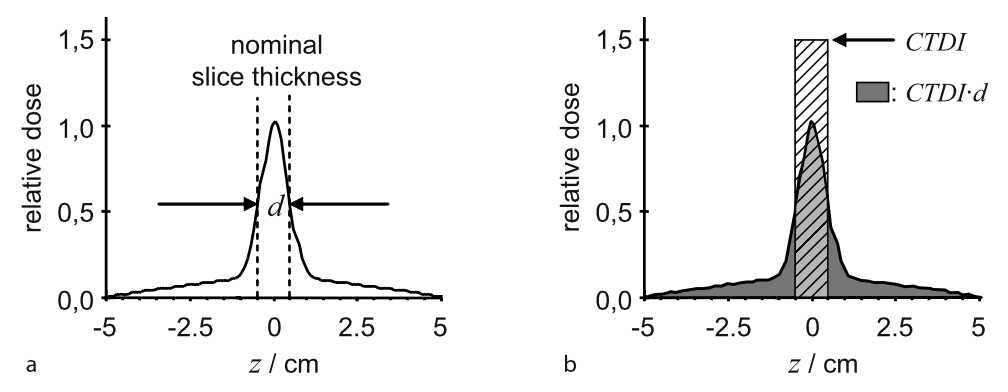
\includegraphics[width=0.8\textwidth]{./figures/ct/dosisprofil.png}
	\caption{a: beobachtetes Dosisprofil einer Schicht der Dicke $d$=\SI{10}{mm} und b: ideales rechteckiges Dosisprofil und \emph{CTDI} als Fläche des Dosisprofils (aus \cite{buzug}, Abb 11.2)}
	\label{fig:ct_dosisprofil}
\end{figure}
Zur einheitlichen Beschreibung der gerätespezifischen Dosis wurde der s.g. \emph{CTDI} (engl. \emph{computed tomography dose index}) eingeführt, der die totale Dosis eines idealerweise rechteckförmigen Dosisprofils entlang der $z$-Achse angibt (wenn die Projektion in der $x$-$y$-Ebene stattfindet)\cite{buzug}.
Er ist definiert als:
\begin{align}
	\text{\emph{CTDI}}=\frac{1}{d}\int_{-\infty}^{+\infty}D(z)\,\mathrm{d}z
\end{align}
Im Rahmen der Strahlenschutzbestimmungen ist es ein ständiges Ziel, die Dosen bei CT-Aufnahmen zu minimieren.
Der Wunsch nach höheren Auflösungen und Kontrasten steht dazu allerdings im Gegensatz, wie die folgenden Überlegungen zeigen, denn die Dosis ist ein entscheidender Faktor der Bildqualität.
Im Rahmen der softwarebasierten Verbesserung der Bildqualität wurde bereits die Nutzung entsprechender Faltungskerne zur Filterung des Signals erwähnt.
Diese können bei gleicher Dosis die Bildschärfe auf Kosten eines steigenden Bildrauschens verbessern oder umgekehrt.
Bei gleichem Signal-Rausch-Verhältnis (\emph{SNR}, engl. \emph{signal-to-noise-ratio}) ist die zur Aufnahme nötige Dosis $D$ proportional zur (mittleren) Transmission des durchstrahlten Objekts\cite{buzug}, so dass für dickere und stärker abschwächende Objekte eine höhere Dosis notwendig ist, um das Bildrauschen gleich zu halten. 
Weiterhin kann gezeigt werden, dass
\begin{align}
	D \propto \frac{(\text{\emph{SNR}})^2}{(\Delta\xi)^4}
\end{align}
gilt, mit $\Delta\xi$ der Größe eines Detektorelements (hier also Aufnahmepixels der Kamera).
Dadurch ergibt sich auch für die Baugröße in Form kleinerer Detektorelemente eine Begrenzung, wenn die Dosis minimiert werden soll.
\section{Fazit}

\FloatBarrier
% BIBLIOGRAPHIE
\vspace{\fill}
% Maximale Anzahl der Einträge in Klammer
% Zitieren mit \cite{lamport94}
\begin{thebibliography}{19}
\bibitem{anleitung}
	Physikalisches Praktikum V: Kern- und Teilchenphysik,
	Versuchsbeschreibung \emph{P523: $\beta$-Spektrometer} (Stand: Januar 2015),
	Universität Bonn	

\bibitem{booklet}
	Center for X-ray Optics and Advanced Light Source,
	\emph{X-Ray Data Booklet}.
	Lawrence Berkeley National Laboratory,
	3. Ausgabe,
	September 2009.

\bibitem{ld_didactic}
	LD Handblätter Physik,
	\emph{P6.3.1.4: Bestimmung der Ionendosisleistung der Röntgenröhre mit Molybdän-Anode}
	
\bibitem{kalender}
	Kalender, W.
	\emph{Computertomographie},
	Publicis Corporate Publishing 2006
	
\bibitem{alkadhi}
	Alkadhi, H.;Leschka, S.;Stolzmann, P.; Scheffel, H.
	\emph{Wie funktioniert CT?},
	Springer 2011
	
\bibitem{buzug}
	Buzug, T.
	\emph{Computed Tomography},
	Springer 2008

\bibitem{riezler}
	Riezler, W.; Kopitzki, K.
	\emph{Kernphysikalisches Praktikum},
	Teubner 1963

\bibitem{nist}
	M. P. Unterweger, D. D. Hoppes, F. J. Schima, J.S. Coursey,
	\emph{NIST Radionuclide Half-Life Measurements},
	\url{http://www.nist.gov/pml/data/halflife-html.cfm} (Letzter Abruf: 1. Mai 2015)

\end{thebibliography}

% APPENDIX
\begin{appendix}
\section{Anhang}

\FloatBarrier
\subsection{Abhängigkeit des Ionisationsstroms von der Kondensatorspannung}
\label{app:ionisationsstrom_kondensatorspannung}
\begin{table}[hp]
	\centering
	\begin{tabular}{SSSSSS}
	\toprule
	{$U_\mathrm{C}/\si{V}$} & {$\Delta U_\mathrm{C}/\si{V}$} & {$U_{I_\mathrm{C}}/\si{mV}$} & {$\Delta U_{I_\mathrm{C}}/\si{mV}$} & {$I_\mathrm{C}/\si{nA}$} & {$\Delta I_\mathrm{C}/\si{nA}$} \\ \midrule
	0.0      & 0.1         & 35        & 5            & 0.035     & 0.006        \\
	5.2      & 0.1         & 115       & 5            & 0.115     & 0.006        \\
	9.7      & 0.1         & 180       & 5            & 0.180     & 0.006        \\
	14.7     & 0.1         & 245       & 5            & 0.245     & 0.006        \\
	19.4     & 0.1         & 290       & 10           & 0.290     & 0.011        \\
	29.7     & 0.1         & 340       & 10           & 0.340     & 0.011        \\
	40.0     & 0.1         & 360       & 10           & 0.360     & 0.011        \\
	49.2     & 0.1         & 390       & 10           & 0.390     & 0.011        \\
	59.0     & 0.1         & 390       & 10           & 0.390     & 0.011        \\
	69.8     & 0.1         & 390       & 10           & 0.390     & 0.011        \\
	80.7     & 0.1         & 395       & 10           & 0.395     & 0.011        \\
	90.3     & 0.1         & 390       & 10           & 0.390     & 0.011        \\
	100.4    & 0.1         & 390       & 10           & 0.390     & 0.011        \\
	119.8    & 0.1         & 380       & 10           & 0.380     & 0.011        \\
	140.4    & 0.1         & 370       & 10           & 0.370     & 0.011        \\
	160.1    & 0.1         & 350       & 10           & 0.350     & 0.011        \\
	179.8    & 0.1         & 340       & 10           & 0.340     & 0.011        \\
	200.3    & 0.1         & 330       & 10           & 0.330     & 0.011        \\
	225.0    & 0.1         & 320       & 10           & 0.320     & 0.011        \\
	250.0    & 0.1         & 310       & 10           & 0.310     & 0.011        \\
	276.1    & 0.1         & 310       & 10           & 0.310     & 0.011        \\
	299.2    & 0.1         & 305       & 10           & 0.305     & 0.011        \\
	325.5    & 0.1         & 305       & 5            & 0.305     & 0.006        \\
	349.6    & 0.1         & 305       & 5            & 0.305     & 0.006        \\
	372.2    & 0.1         & 305       & 5            & 0.305     & 0.006        \\ \bottomrule
\end{tabular}
	\caption{Zusammenhang von Ionisationsstrom $I_\mathrm{C}$, welcher anhand des Spannungsabfalls $U_{I_\mathrm{C}}$ an einem Messwiderstand $R = \SI{1.00+-0.01}{\giga\ohm}$ gemessen wurde und Kondensatorspannung $U_\mathrm{C}$. Die Röntgenröhrenspannung der Molybdän-Röhre wurde auf $U = \SI{15}{kV}$ und der Emissionsstrom auf $I_\mathrm{E} = \SI{1.00}{mA}$ eingestellt.}
	\label{tab:kondensatorspannung_15kV}
\end{table}
\begin{table}[hp]
	\centering
	\begin{tabular}{SSSSSS}
	\toprule
	{$U_\mathrm{C}/\si{V}$} & {$\Delta U_\mathrm{C}/\si{V}$} & {$U_{I_\mathrm{C}}/\si{mV}$} & {$\Delta U_{I_\mathrm{C}}/\si{mV}$} & {$I_\mathrm{C}/\si{nA}$} & {$\Delta I_\mathrm{C}/\si{nA}$} \\ \midrule
	0.0   & 0.1 & 30   & 5  & 0.030 & 0.006 \\
	5.7   & 0.1 & 240  & 10 & 0.240 & 0.011 \\
	10.1  & 0.1 & 410  & 10 & 0.410 & 0.011 \\
	15.0  & 0.1 & 600  & 10 & 0.600 & 0.012 \\
	19.8  & 0.1 & 810  & 10 & 0.810 & 0.013 \\
	25.5  & 0.1 & 1050 & 20 & 1.050 & 0.023 \\
	30.3  & 0.1 & 1230 & 20 & 1.230 & 0.024 \\
	34.1  & 0.1 & 1360 & 20 & 1.360 & 0.025 \\
	40.4  & 0.1 & 1580 & 20 & 1.580 & 0.026 \\
	45.4  & 0.1 & 1690 & 20 & 1.690 & 0.027 \\
	49.1  & 0.1 & 1770 & 20 & 1.770 & 0.027 \\
	59.5  & 0.1 & 1920 & 20 & 1.920 & 0.028 \\
	70.3  & 0.1 & 1980 & 20 & 1.980 & 0.029 \\
	81.3  & 0.1 & 2060 & 20 & 2.060 & 0.029 \\
	89.4  & 0.1 & 2090 & 20 & 2.090 & 0.029 \\
	101.0 & 0.1 & 2110 & 20 & 2.110 & 0.030 \\
	120.2 & 0.1 & 2130 & 20 & 2.130 & 0.030 \\
	141.6 & 0.1 & 2130 & 10 & 2.130 & 0.024 \\
	159.9 & 0.1 & 2140 & 10 & 2.140 & 0.024 \\
	179.5 & 0.1 & 2115 & 10 & 2.115 & 0.024 \\
	200.3 & 0.1 & 2110 & 10 & 2.110 & 0.024 \\
	226.0 & 0.1 & 2070 & 10 & 2.070 & 0.023 \\
	251.2 & 0.1 & 2030 & 10 & 2.030 & 0.023 \\
	276.1 & 0.1 & 2010 & 10 & 2.010 & 0.023 \\
	300.2 & 0.1 & 2020 & 10 & 2.020 & 0.023 \\
	325.3 & 0.1 & 2000 & 10 & 2.000 & 0.023 \\
	351.3 & 0.1 & 1990 & 10 & 1.990 & 0.023 \\
	371.5 & 0.1 & 1990 & 10 & 1.990 & 0.023 \\ \bottomrule
\end{tabular}

	\caption{Zusammenhang von Ionisationsstrom $I_\mathrm{C}$, welcher anhand des Spannungsabfalls $U_{I_\mathrm{C}}$ an einem Messwiderstand $R = \SI{1.00+-0.01}{\giga\ohm}$ gemessen wurde und Kondensatorspannung $U_\mathrm{C}$. Die Röntgenröhrenspannung der Molybdän-Röhre wurde auf $U = \SI{25}{kV}$ und der Emissionsstrom auf $I_\mathrm{E} = \SI{1.00}{mA}$ eingestellt.}
	\label{tab:kondensatorspannung_25kV}
\end{table}
\begin{table}[hp]
	\centering
	\begin{tabular}{SSSSSS}
	\toprule
	{$U_\mathrm{C}/\si{V}$} & {$\Delta U_\mathrm{C}/\si{V}$} & {$U_{I_\mathrm{C}}/\si{mV}$} & {$\Delta U_{I_\mathrm{C}}/\si{mV}$} & {$I_\mathrm{C}/\si{nA}$} & {$\Delta I_\mathrm{C}/\si{nA}$} \\ \midrule
	0.0   & 0.1 & 30   & 10 & 0.030 & 0.011 \\
	5.2   & 0.1 & 300  & 20 & 0.300 & 0.021 \\
	9.5   & 0.1 & 550  & 20 & 0.550 & 0.021 \\
	14.2  & 0.1 & 810  & 10 & 0.810 & 0.013 \\
	19.9  & 0.1 & 1160 & 10 & 1.160 & 0.016 \\
	24.8  & 0.1 & 1480 & 10 & 1.480 & 0.018 \\
	29.2  & 0.1 & 1760 & 10 & 1.760 & 0.021 \\
	35.9  & 0.1 & 2180 & 10 & 2.180 & 0.024 \\
	40.5  & 0.1 & 2490 & 10 & 2.490 & 0.027 \\
	44.6  & 0.1 & 2730 & 10 & 2.730 & 0.030 \\
	49.1  & 0.1 & 3020 & 10 & 3.020 & 0.032 \\
	60.6  & 0.1 & 3640 & 10 & 3.640 & 0.038 \\
	68.8  & 0.1 & 3960 & 20 & 3.960 & 0.045 \\
	80.4  & 0.1 & 4330 & 20 & 4.330 & 0.048 \\
	89.0  & 0.1 & 4480 & 20 & 4.480 & 0.050 \\
	100.9 & 0.1 & 4680 & 20 & 4.680 & 0.051 \\
	119.0 & 0.1 & 4820 & 20 & 4.820 & 0.053 \\
	139.7 & 0.1 & 4970 & 20 & 4.970 & 0.054 \\
	159.9 & 0.1 & 5000 & 20 & 5.000 & 0.054 \\
	182.9 & 0.1 & 5000 & 20 & 5.000 & 0.054 \\
	202.0 & 0.1 & 5020 & 20 & 5.020 & 0.055 \\
	218.3 & 0.1 & 5050 & 50 & 5.050 & 0.072 \\
	243.7 & 0.1 & 5020 & 50 & 5.020 & 0.071 \\
	261.1 & 0.1 & 5000 & 50 & 5.000 & 0.071 \\
	280.0 & 0.1 & 4990 & 20 & 4.990 & 0.054 \\
	300.5 & 0.1 & 4980 & 20 & 4.980 & 0.054 \\
	326.0 & 0.1 & 4970 & 20 & 4.970 & 0.054 \\
	350.3 & 0.1 & 4950 & 20 & 4.950 & 0.054 \\
	374.6 & 0.1 & 4930 & 20 & 4.930 & 0.054 \\ \bottomrule
\end{tabular}
	\caption{Zusammenhang von Ionisationsstrom $I_\mathrm{C}$, welcher anhand des Spannungsabfalls $U_{I_\mathrm{C}}$ an einem Messwiderstand $R = \SI{1.00+-0.01}{\giga\ohm}$ gemessen wurde und Kondensatorspannung $U_\mathrm{C}$. Die Röntgenröhrenspannung der Molybdän-Röhre wurde auf $U = \SI{35}{kV}$ und der Emissionsstrom auf $I_\mathrm{E} = \SI{1.00}{mA}$ eingestellt.}
	\label{tab:kondensatorspannung_35kV}
\end{table}
\FloatBarrier

\subsection{Abhängigkeit des Ionisationsstroms von dem Emissionsstrom}
\label{app:ionisationsstrom_emissionsstrom}
\begin{table}[hp]
	\centering
	\begin{subtable}[c]{0.75\textwidth}
		% GNUPLOT: LaTeX picture with Postscript
\begingroup
  \makeatletter
  \providecommand\color[2][]{%
    \GenericError{(gnuplot) \space\space\space\@spaces}{%
      Package color not loaded in conjunction with
      terminal option `colourtext'%
    }{See the gnuplot documentation for explanation.%
    }{Either use 'blacktext' in gnuplot or load the package
      color.sty in LaTeX.}%
    \renewcommand\color[2][]{}%
  }%
  \providecommand\includegraphics[2][]{%
    \GenericError{(gnuplot) \space\space\space\@spaces}{%
      Package graphicx or graphics not loaded%
    }{See the gnuplot documentation for explanation.%
    }{The gnuplot epslatex terminal needs graphicx.sty or graphics.sty.}%
    \renewcommand\includegraphics[2][]{}%
  }%
  \providecommand\rotatebox[2]{#2}%
  \@ifundefined{ifGPcolor}{%
    \newif\ifGPcolor
    \GPcolortrue
  }{}%
  \@ifundefined{ifGPblacktext}{%
    \newif\ifGPblacktext
    \GPblacktexttrue
  }{}%
  % define a \g@addto@macro without @ in the name:
  \let\gplgaddtomacro\g@addto@macro
  % define empty templates for all commands taking text:
  \gdef\gplbacktext{}%
  \gdef\gplfronttext{}%
  \makeatother
  \ifGPblacktext
    % no textcolor at all
    \def\colorrgb#1{}%
    \def\colorgray#1{}%
  \else
    % gray or color?
    \ifGPcolor
      \def\colorrgb#1{\color[rgb]{#1}}%
      \def\colorgray#1{\color[gray]{#1}}%
      \expandafter\def\csname LTw\endcsname{\color{white}}%
      \expandafter\def\csname LTb\endcsname{\color{black}}%
      \expandafter\def\csname LTa\endcsname{\color{black}}%
      \expandafter\def\csname LT0\endcsname{\color[rgb]{1,0,0}}%
      \expandafter\def\csname LT1\endcsname{\color[rgb]{0,1,0}}%
      \expandafter\def\csname LT2\endcsname{\color[rgb]{0,0,1}}%
      \expandafter\def\csname LT3\endcsname{\color[rgb]{1,0,1}}%
      \expandafter\def\csname LT4\endcsname{\color[rgb]{0,1,1}}%
      \expandafter\def\csname LT5\endcsname{\color[rgb]{1,1,0}}%
      \expandafter\def\csname LT6\endcsname{\color[rgb]{0,0,0}}%
      \expandafter\def\csname LT7\endcsname{\color[rgb]{1,0.3,0}}%
      \expandafter\def\csname LT8\endcsname{\color[rgb]{0.5,0.5,0.5}}%
    \else
      % gray
      \def\colorrgb#1{\color{black}}%
      \def\colorgray#1{\color[gray]{#1}}%
      \expandafter\def\csname LTw\endcsname{\color{white}}%
      \expandafter\def\csname LTb\endcsname{\color{black}}%
      \expandafter\def\csname LTa\endcsname{\color{black}}%
      \expandafter\def\csname LT0\endcsname{\color{black}}%
      \expandafter\def\csname LT1\endcsname{\color{black}}%
      \expandafter\def\csname LT2\endcsname{\color{black}}%
      \expandafter\def\csname LT3\endcsname{\color{black}}%
      \expandafter\def\csname LT4\endcsname{\color{black}}%
      \expandafter\def\csname LT5\endcsname{\color{black}}%
      \expandafter\def\csname LT6\endcsname{\color{black}}%
      \expandafter\def\csname LT7\endcsname{\color{black}}%
      \expandafter\def\csname LT8\endcsname{\color{black}}%
    \fi
  \fi
    \setlength{\unitlength}{0.0500bp}%
    \ifx\gptboxheight\undefined%
      \newlength{\gptboxheight}%
      \newlength{\gptboxwidth}%
      \newsavebox{\gptboxtext}%
    \fi%
    \setlength{\fboxrule}{0.5pt}%
    \setlength{\fboxsep}{1pt}%
\begin{picture}(7200.00,5040.00)%
    \gplgaddtomacro\gplbacktext{%
      \csname LTb\endcsname%
      \put(550,704){\makebox(0,0)[r]{\strut{}$0$}}%
      \csname LTb\endcsname%
      \put(550,1383){\makebox(0,0)[r]{\strut{}$1$}}%
      \csname LTb\endcsname%
      \put(550,2061){\makebox(0,0)[r]{\strut{}$2$}}%
      \csname LTb\endcsname%
      \put(550,2740){\makebox(0,0)[r]{\strut{}$3$}}%
      \csname LTb\endcsname%
      \put(550,3418){\makebox(0,0)[r]{\strut{}$4$}}%
      \csname LTb\endcsname%
      \put(550,4097){\makebox(0,0)[r]{\strut{}$5$}}%
      \csname LTb\endcsname%
      \put(550,4775){\makebox(0,0)[r]{\strut{}$6$}}%
      \csname LTb\endcsname%
      \put(682,484){\makebox(0,0){\strut{}$0$}}%
      \csname LTb\endcsname%
      \put(1906,484){\makebox(0,0){\strut{}$0{,}2$}}%
      \csname LTb\endcsname%
      \put(3130,484){\makebox(0,0){\strut{}$0{,}4$}}%
      \csname LTb\endcsname%
      \put(4355,484){\makebox(0,0){\strut{}$0{,}6$}}%
      \csname LTb\endcsname%
      \put(5579,484){\makebox(0,0){\strut{}$0{,}8$}}%
      \csname LTb\endcsname%
      \put(6803,484){\makebox(0,0){\strut{}$1$}}%
    }%
    \gplgaddtomacro\gplfronttext{%
      \csname LTb\endcsname%
      \put(176,2739){\rotatebox{-270}{\makebox(0,0){\strut{}Ionisationsstrom $I_\mathrm{C} / \si{nA}$}}}%
      \put(3742,154){\makebox(0,0){\strut{}Emissionsstrom $I_\mathrm{E} / \si{mA}$}}%
      \csname LTb\endcsname%
      \put(2002,4602){\makebox(0,0)[r]{\strut{}Messdaten}}%
      \csname LTb\endcsname%
      \put(2002,4382){\makebox(0,0)[r]{\strut{}Anpassung}}%
    }%
    \gplbacktext
    \put(0,0){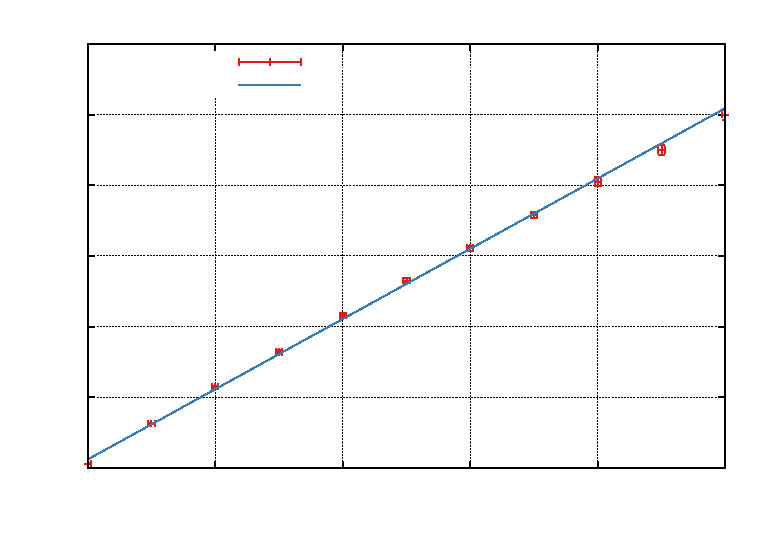
\includegraphics{./plots/abh_emissionsstrom/mo}}%
    \gplfronttext
  \end{picture}%
\endgroup

		\subcaption{Molybdän-Röhre mit Messwiderstand $R = \SI{1.00+-0.01}{\giga\ohm}$}
		\label{tab:emissionsstrom_mo}
	\end{subtable}
	
	\vspace{10mm}
	
	\begin{subtable}[c]{0.75\textwidth}
		\begin{tabular}{SSSSSS}
	\toprule
	{$U / \si{kV}$} & {$\Delta U / \si{kV}$} & {$U_{I_\mathrm{C}} / \si{mV}$} & {$\Delta U_{I_\mathrm{C}} / \si{mV}$} & {$I_\mathrm{C} / \si{nA}$} & {$\Delta I_\mathrm{C} / \si{nA}$} \\ \midrule
	0.00   & 0.05      & 13        & 2            & 0.13      & 0.03         \\
	2.50   & 0.05      & 13        & 2            & 0.13      & 0.03         \\
	5.00   & 0.05      & 38        & 2            & 0.38      & 0.03         \\
	7.50   & 0.05      & 180       & 5            & 1.80      & 0.06         \\
	10.00  & 0.05      & 550       & 10           & 5.50      & 0.12         \\
	12.50  & 0.05      & 1090      & 10           & 10.90     & 0.15         \\
	15.00  & 0.05      & 1700      & 10           & 17.00     & 0.20         \\
	17.50  & 0.05      & 2330      & 10           & 23.30     & 0.26         \\
	20.00  & 0.05      & 2960      & 10           & 29.60     & 0.32         \\
	22.50  & 0.05      & 3510      & 10           & 35.10     & 0.37         \\
	25.00  & 0.05      & 3990      & 10           & 39.90     & 0.42         \\
	27.50  & 0.05      & 4390      & 10           & 43.90     & 0.46         \\
	30.00  & 0.05      & 4730      & 10           & 47.30     & 0.49         \\
	32.50  & 0.05      & 5020      & 10           & 50.20     & 0.52         \\
	35.00  & 0.05      & 5260      & 20           & 52.60     & 0.57         \\ \bottomrule
\end{tabular}
		\subcaption{Kupfer-Röhre mit Messwiderstand $R = \SI{100 +- 1}{\mega\ohm}$}
		\label{tab:emissionsstrom_cu}
	\end{subtable}	
	\caption{Gemessener Zusammenhang zwischen Emissionsstrom $I_\mathrm{E}$ der Röntgenröhre und Ionisationsstrom $I_\mathrm{C}$. Der Ionisationsstrom wurde als Spannungsabfall $U_{I_\mathrm{C}}$ über einem Messwiderstand $R$ gemessen.}
\end{table}
\FloatBarrier

\subsection{Abhängigkeit des Ionisationsstroms von der Röhrenspannung}
\label{app:ionisationsstrom_roehrenspannung}
\begin{table}[hp]
	\centering
	\begin{subtable}[c]{0.75\textwidth}
		% GNUPLOT: LaTeX picture with Postscript
\begingroup
  \makeatletter
  \providecommand\color[2][]{%
    \GenericError{(gnuplot) \space\space\space\@spaces}{%
      Package color not loaded in conjunction with
      terminal option `colourtext'%
    }{See the gnuplot documentation for explanation.%
    }{Either use 'blacktext' in gnuplot or load the package
      color.sty in LaTeX.}%
    \renewcommand\color[2][]{}%
  }%
  \providecommand\includegraphics[2][]{%
    \GenericError{(gnuplot) \space\space\space\@spaces}{%
      Package graphicx or graphics not loaded%
    }{See the gnuplot documentation for explanation.%
    }{The gnuplot epslatex terminal needs graphicx.sty or graphics.sty.}%
    \renewcommand\includegraphics[2][]{}%
  }%
  \providecommand\rotatebox[2]{#2}%
  \@ifundefined{ifGPcolor}{%
    \newif\ifGPcolor
    \GPcolortrue
  }{}%
  \@ifundefined{ifGPblacktext}{%
    \newif\ifGPblacktext
    \GPblacktexttrue
  }{}%
  % define a \g@addto@macro without @ in the name:
  \let\gplgaddtomacro\g@addto@macro
  % define empty templates for all commands taking text:
  \gdef\gplbacktext{}%
  \gdef\gplfronttext{}%
  \makeatother
  \ifGPblacktext
    % no textcolor at all
    \def\colorrgb#1{}%
    \def\colorgray#1{}%
  \else
    % gray or color?
    \ifGPcolor
      \def\colorrgb#1{\color[rgb]{#1}}%
      \def\colorgray#1{\color[gray]{#1}}%
      \expandafter\def\csname LTw\endcsname{\color{white}}%
      \expandafter\def\csname LTb\endcsname{\color{black}}%
      \expandafter\def\csname LTa\endcsname{\color{black}}%
      \expandafter\def\csname LT0\endcsname{\color[rgb]{1,0,0}}%
      \expandafter\def\csname LT1\endcsname{\color[rgb]{0,1,0}}%
      \expandafter\def\csname LT2\endcsname{\color[rgb]{0,0,1}}%
      \expandafter\def\csname LT3\endcsname{\color[rgb]{1,0,1}}%
      \expandafter\def\csname LT4\endcsname{\color[rgb]{0,1,1}}%
      \expandafter\def\csname LT5\endcsname{\color[rgb]{1,1,0}}%
      \expandafter\def\csname LT6\endcsname{\color[rgb]{0,0,0}}%
      \expandafter\def\csname LT7\endcsname{\color[rgb]{1,0.3,0}}%
      \expandafter\def\csname LT8\endcsname{\color[rgb]{0.5,0.5,0.5}}%
    \else
      % gray
      \def\colorrgb#1{\color{black}}%
      \def\colorgray#1{\color[gray]{#1}}%
      \expandafter\def\csname LTw\endcsname{\color{white}}%
      \expandafter\def\csname LTb\endcsname{\color{black}}%
      \expandafter\def\csname LTa\endcsname{\color{black}}%
      \expandafter\def\csname LT0\endcsname{\color{black}}%
      \expandafter\def\csname LT1\endcsname{\color{black}}%
      \expandafter\def\csname LT2\endcsname{\color{black}}%
      \expandafter\def\csname LT3\endcsname{\color{black}}%
      \expandafter\def\csname LT4\endcsname{\color{black}}%
      \expandafter\def\csname LT5\endcsname{\color{black}}%
      \expandafter\def\csname LT6\endcsname{\color{black}}%
      \expandafter\def\csname LT7\endcsname{\color{black}}%
      \expandafter\def\csname LT8\endcsname{\color{black}}%
    \fi
  \fi
    \setlength{\unitlength}{0.0500bp}%
    \ifx\gptboxheight\undefined%
      \newlength{\gptboxheight}%
      \newlength{\gptboxwidth}%
      \newsavebox{\gptboxtext}%
    \fi%
    \setlength{\fboxrule}{0.5pt}%
    \setlength{\fboxsep}{1pt}%
\begin{picture}(7200.00,5040.00)%
    \gplgaddtomacro\gplbacktext{%
      \csname LTb\endcsname%
      \put(550,704){\makebox(0,0)[r]{\strut{}$0$}}%
      \csname LTb\endcsname%
      \put(550,1383){\makebox(0,0)[r]{\strut{}$1$}}%
      \csname LTb\endcsname%
      \put(550,2061){\makebox(0,0)[r]{\strut{}$2$}}%
      \csname LTb\endcsname%
      \put(550,2740){\makebox(0,0)[r]{\strut{}$3$}}%
      \csname LTb\endcsname%
      \put(550,3418){\makebox(0,0)[r]{\strut{}$4$}}%
      \csname LTb\endcsname%
      \put(550,4097){\makebox(0,0)[r]{\strut{}$5$}}%
      \csname LTb\endcsname%
      \put(550,4775){\makebox(0,0)[r]{\strut{}$6$}}%
      \csname LTb\endcsname%
      \put(682,484){\makebox(0,0){\strut{}$0$}}%
      \csname LTb\endcsname%
      \put(1906,484){\makebox(0,0){\strut{}$0{,}2$}}%
      \csname LTb\endcsname%
      \put(3130,484){\makebox(0,0){\strut{}$0{,}4$}}%
      \csname LTb\endcsname%
      \put(4355,484){\makebox(0,0){\strut{}$0{,}6$}}%
      \csname LTb\endcsname%
      \put(5579,484){\makebox(0,0){\strut{}$0{,}8$}}%
      \csname LTb\endcsname%
      \put(6803,484){\makebox(0,0){\strut{}$1$}}%
    }%
    \gplgaddtomacro\gplfronttext{%
      \csname LTb\endcsname%
      \put(176,2739){\rotatebox{-270}{\makebox(0,0){\strut{}Ionisationsstrom $I_\mathrm{C} / \si{nA}$}}}%
      \put(3742,154){\makebox(0,0){\strut{}Emissionsstrom $I_\mathrm{E} / \si{mA}$}}%
      \csname LTb\endcsname%
      \put(2002,4602){\makebox(0,0)[r]{\strut{}Messdaten}}%
      \csname LTb\endcsname%
      \put(2002,4382){\makebox(0,0)[r]{\strut{}Anpassung}}%
    }%
    \gplbacktext
    \put(0,0){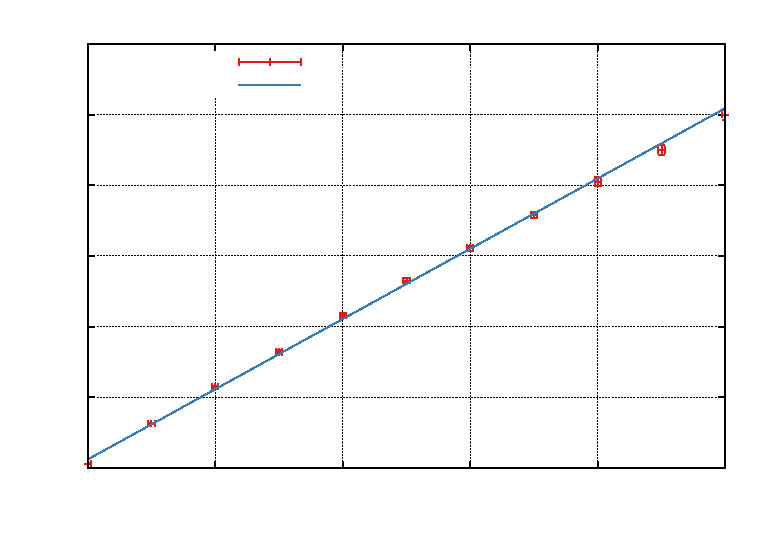
\includegraphics{./plots/abh_emissionsstrom/mo}}%
    \gplfronttext
  \end{picture}%
\endgroup

		\subcaption{Molybdän-Röhre mit Messwiderstand $R = \SI{1.00+-0.01}{\giga\ohm}$}
		\label{tab:roehrenspannung_mo}
	\end{subtable}
	
	\vspace{10mm}
	
	\begin{subtable}[c]{0.75\textwidth}
		\begin{tabular}{SSSSSS}
	\toprule
	{$U / \si{kV}$} & {$\Delta U / \si{kV}$} & {$U_{I_\mathrm{C}} / \si{mV}$} & {$\Delta U_{I_\mathrm{C}} / \si{mV}$} & {$I_\mathrm{C} / \si{nA}$} & {$\Delta I_\mathrm{C} / \si{nA}$} \\ \midrule
	0.00   & 0.05      & 13        & 2            & 0.13      & 0.03         \\
	2.50   & 0.05      & 13        & 2            & 0.13      & 0.03         \\
	5.00   & 0.05      & 38        & 2            & 0.38      & 0.03         \\
	7.50   & 0.05      & 180       & 5            & 1.80      & 0.06         \\
	10.00  & 0.05      & 550       & 10           & 5.50      & 0.12         \\
	12.50  & 0.05      & 1090      & 10           & 10.90     & 0.15         \\
	15.00  & 0.05      & 1700      & 10           & 17.00     & 0.20         \\
	17.50  & 0.05      & 2330      & 10           & 23.30     & 0.26         \\
	20.00  & 0.05      & 2960      & 10           & 29.60     & 0.32         \\
	22.50  & 0.05      & 3510      & 10           & 35.10     & 0.37         \\
	25.00  & 0.05      & 3990      & 10           & 39.90     & 0.42         \\
	27.50  & 0.05      & 4390      & 10           & 43.90     & 0.46         \\
	30.00  & 0.05      & 4730      & 10           & 47.30     & 0.49         \\
	32.50  & 0.05      & 5020      & 10           & 50.20     & 0.52         \\
	35.00  & 0.05      & 5260      & 20           & 52.60     & 0.57         \\ \bottomrule
\end{tabular}
		\subcaption{Kupfer-Röhre mit Messwiderstand $R = \SI{100+-1}{\mega\ohm}$}
		\label{tab:roehrenspannung_cu}
	\end{subtable}	
	\caption{Gemessener Zusammenhang zwischen Röhrenspannung $U$ und Ionisationsstrom $I_\mathrm{C}$. Der Ionisationsstrom wurde als Spannungsabfall $U_{I_\mathrm{C}}$ über einem Messwiderstand $R$ gemessen.}
\end{table}
\FloatBarrier

\end{appendix}

\end{document}
